% Abbildung, die nach und nach wächst, mit den erklärten Teilbereichen

% vgl IPCC AR5 climate feedbacks, AR4 chapter 1 basics: carbon cycle
\subsection{Die Faktoren des Klimasystems}

\begin{frame}
  \frametitle{Faktoren des Klimasystems}
  \begin{columns}
	\column{0.7\linewidth}
	\begin{figure}
	 	\centering
    % trim={<left> <lower> <right> <upper>}
	 	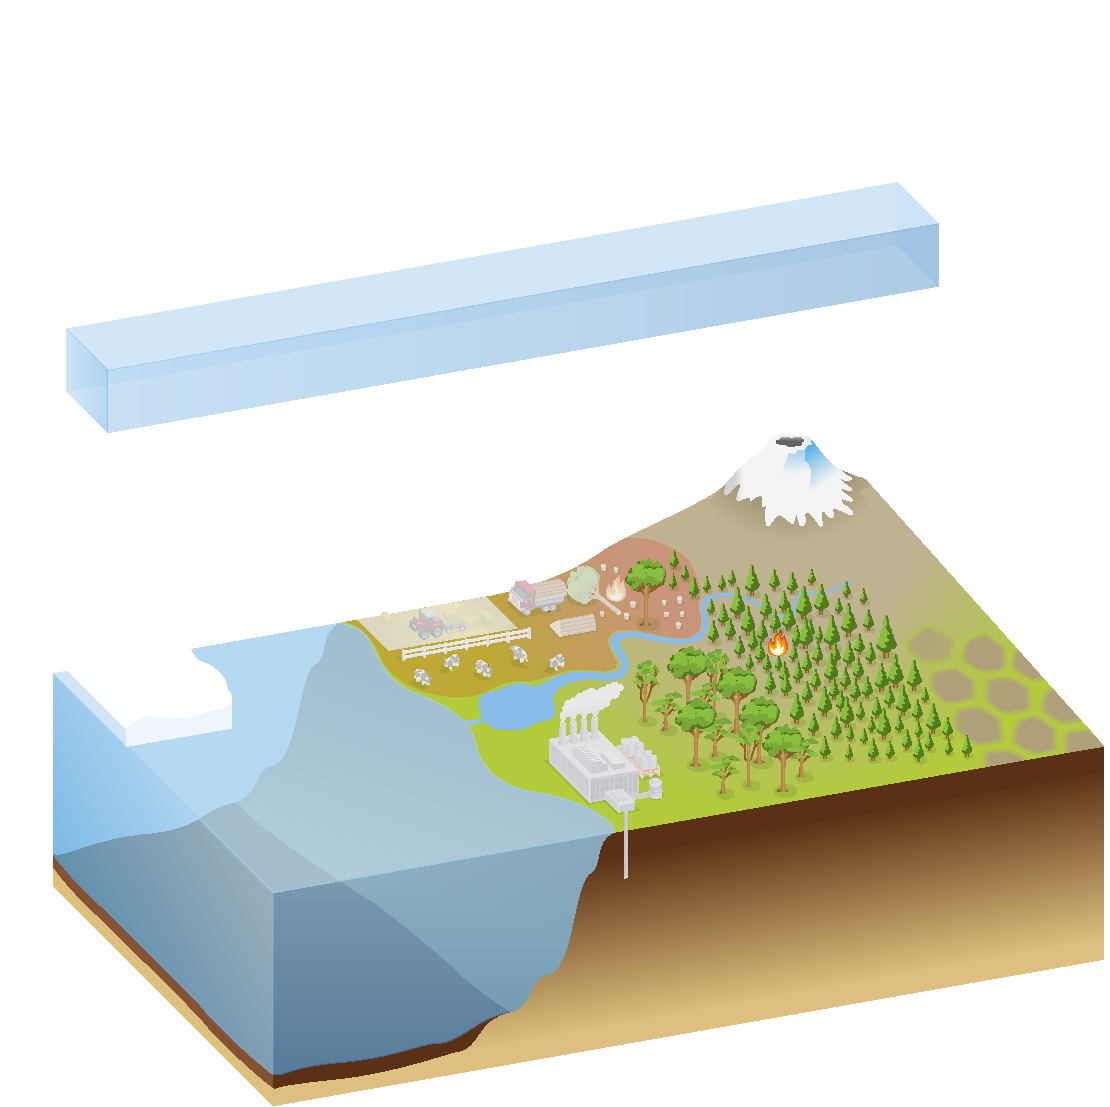
\includegraphics[trim={1cm 0cm 0cm 3cm}, clip, width=0.8\linewidth]{%
        bilder/climate_components/global_climate_components_spheres_ex_human.pdf}
	 	\caption{Schematische Abbildung des Klimasystems, Quelle: IPCC 2013, Physical Science Base, Kapitel 6} % Anmerkungen hinzugefügt nach
	\end{figure}
  \column{0.3\linewidth}
  \textbf{Sphären des Klimasystems}\\
  (altgriechisch)\\[1em]
  \textit{atmos} = Dunst\\
  \textit{hydor} = Wasser\\
  \textit{kryos} = Eis\\
  \textit{bios} = Leben\\
  \textit{pedon} = Boden\\
  \textit{lithos} = Stein
	%TODO: Evtl Bezeichnungen in Bild einfügen anstatt separat auflisten
	\end{columns}

	\note{
	\begin{itemize}
    \item[] Sphären
    \begin{itemize}
      \item[] Atmosphäre: Gasförmige Hülle der Erde\\
      \item[] Hydrosphäre: Ozeane, sowie Wasserkreislauf auf den Kontinenten
              und in der Atmosphäre\\
      \item[] Kryosphäre: Schnee und Eis\\
      \item[] Biosphäre: Lebewesen, Tiere und Pflanzen\\
      \item[] Pedosphäre: Boden\\
      \item[] Lithosphäre: Gestein
    \end{itemize}
		\item[] Hier: Vorstellung aller Sphären, sowie einiger wichtiger Interaktionen zwischen ihnen.
		\item[] Die Effekte des Klimawandels sind bereits heute spürbar: Dürreperioden und Überflutungen, Rückgang der Eisschilde und Waldrodung.
		\item[] Die Zustände der Böden sind entscheidend für die Vegetation und Landwirtschaft.
		\item[] $\rightarrow$ Erosion von Böden durch Übernutzung und Dürren macht sie unfruchtbar (Nährstoffverlust und Austrocknung).
		\item[] $\rightarrow$ Gestein liefert Mineralien, was ebenfalls für die Vegetation und auch z.B. Schalenbildung bei Muscheln wichtig ist.
	\end{itemize}
	}
\end{frame}

\begin{frame}
	\frametitle{Atmosphäre - Luftmassen}

	\begin{figure}
		\centering
		\begin{tikzpicture}
			\node (image1) {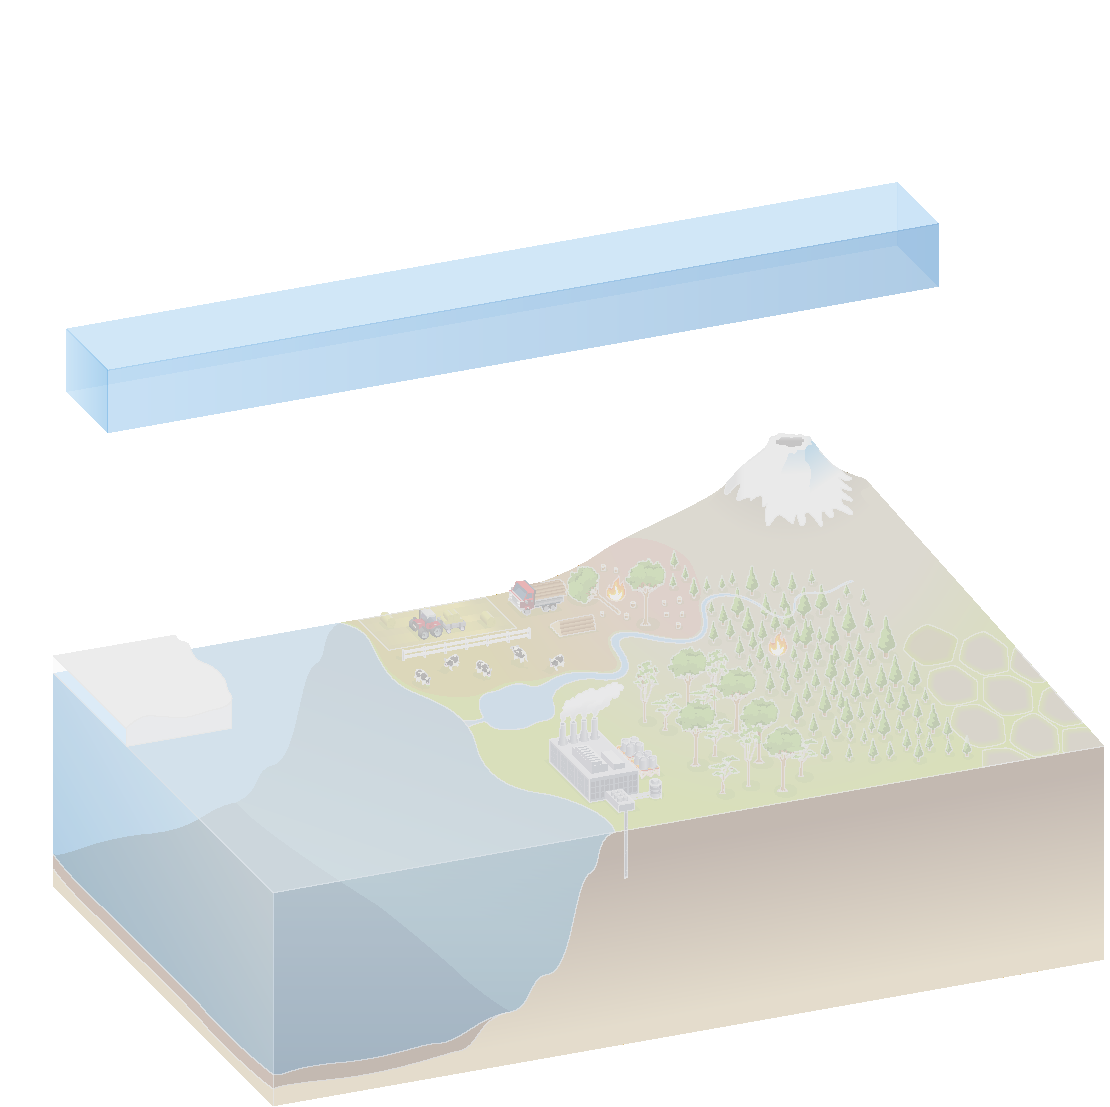
\includegraphics[trim={1cm 0cm 0cm 3cm}, clip, width=0.55\linewidth]{%
        	bilder/climate_components/global_climate_components_atmosphere.pdf}};
			\onslide<2|handout:0>\node (image2) at (image1.east) [xshift=-0.9cm]{%
					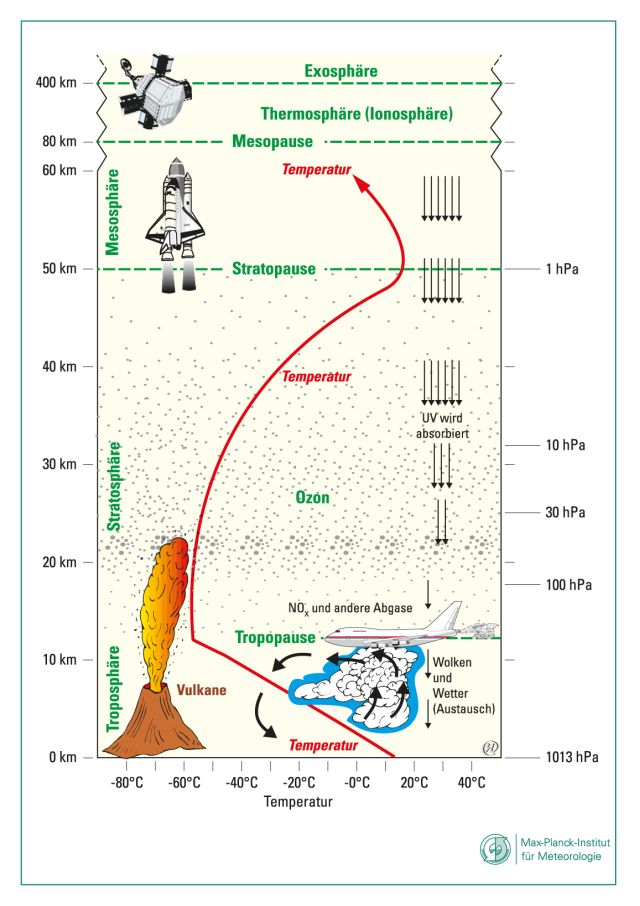
\includegraphics[width=0.35\linewidth] der Atmosphärenmasse, enthält fast allen Wasserdampf
			    \item[] Hier finden alle wetterrelevanten Phänomene statt
			  \end{itemize}
			  \item Stratosphäre, \SIrange{12}{50}{km}, \SIrange{-60}{0}{\celsius}, Ozon sorgt für Temperaturanstieg durch UV-Absorption
			  \item Mesosphäre, \SIrange{50}{80}{km}, \SIrange{-100}{0}{\celsius}, Temperatur fällt
			  \item Thermosphäre, \SIrange{80}{400}{km}, extrem geringe Teilchendichte, daher Temperatur nicht bestimmbar, Weltraum
			  \item Exosphäre, \SIrange{400}{1000}{km}, quasi Vakuum
			\end{itemize}
			\item[] Passt sich am schnellsten an Änderungen an $\rightarrow$ Wie funktionieren die Ausgleichsprozesse?
			\item[] in der planetaren Grenzschicht (\SIrange{1}{2.5}{km}): Reibung wichtig $\rightarrow$ starke vertikale Unterschiede in diesem Bereich der Atmosphäre
		\end{itemize}
		}
\end{frame}

\begin{frame}
	\frametitle{Globale Atmosphärische Zirkulation}

	\begin{figure}
		\centering
		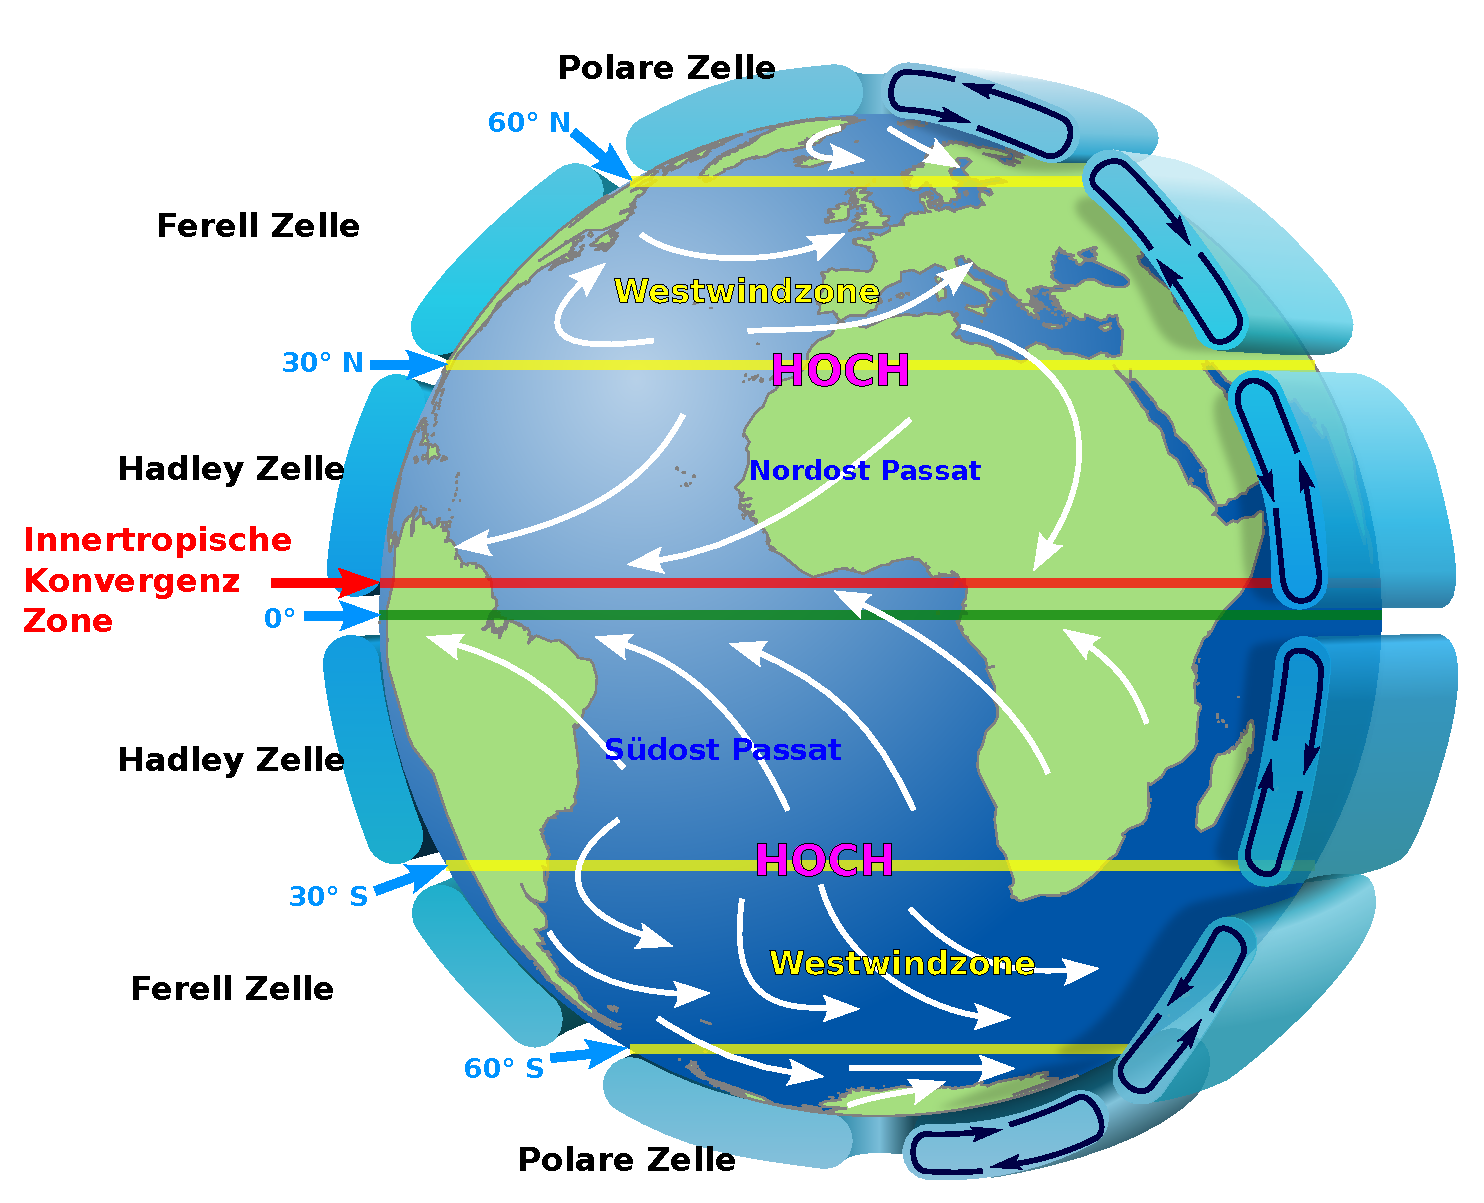
\includegraphics[width=.65\linewidth]{bilder/Earth_Global_Circulation_-_de.pdf}
		\caption{Globale atmosphärische Zirkulation, Quelle: MireRun/Kaidor nach NASA Global circulation of Earth's atmosphere}
	\end{figure}

	\note{
	Großskalige Modellvorstellung globaler Zirkulationssysteme in der Atmosphäre

	Starke Vereinfachung:
		\begin{itemize}
			\item[] Am Äquator steigt warme Luft auf, hinterlässt ein Tiefdruckgebiet (weniger Luft vorhanden).
    	\item[] In Bodennähe strömt kältere Luft in Richtung Äquator nach.
			\item[] Wegen der Drehung der Erde (Corioliskraft) werden Bewegungen auf der Nordhalbkugel im Uhrzeigersinn abgelenkt, auf der Südhalbkugel gegen den Uhrzeigersinn. Eine äquatorwärts strömende Luftmasse wird dadurch auf der Nordhalbkugel zum Nordostwind, auf der Südhalbkugel zum Südostwind.
			\item[] In der Höhe kommt es zu Ausgleichsströmungen: Luftmassen, die über dem Äquator aufgestiegen sind, strömen in der Höhe wieder polwärts. Am Pol in der Höhe eintreffende Luftmassen sinken dort ab.
		\end{itemize}

		Etwas genauer:
		\begin{itemize}
			\item[] vom Äquator weg strömende Luftmassen, sinken wegen der polwärtigen Flächenkonvergenz der Erde über rund \SI{30}{\degree} Breite wieder ab (Hadley Zelle, Passatwinde).
			\item[] vom Pol weg strömende Luftmassen, erwärmen sich, steigen ab rund \SI{60}{\degree} Breite wieder auf (Polare Zelle).
    	\item[] Zwischen beiden Systemen jeder Hemisphäre jeweils ein dritte, gegenläufige Zelle (Ferell Zelle, Westwinde).
    	\item[$\rightarrow$] Sowohl auf der Nord- als auch auf der Südhalbkugel jeweils drei (bodennahe) Windsysteme,
			\item[] Innertropische Konvergenzzone trennt Nord- und Südhalbkugel, Tiefdruckrinne
		\end{itemize}
		\begin{itemize}
			\item[Hadley Z.] Passatwinde sehr stabil, zur schnellen Überquerung der Ozeane genutzt
			\item[Polare Z.] Sehr stabil
			\item[Ferell Z.] instabil, gegenläufig zu polarer Zelle und Hadley Zelle. Enthält ca. \SI{38}{\percent} der Energieunterschiede zwischen Pol und Äquator.
		\end{itemize}
	}
\end{frame}

\begin{frame}
	\frametitle{Hydrosphäre - Wassermassen}
	\begin{figure}
		\centering
		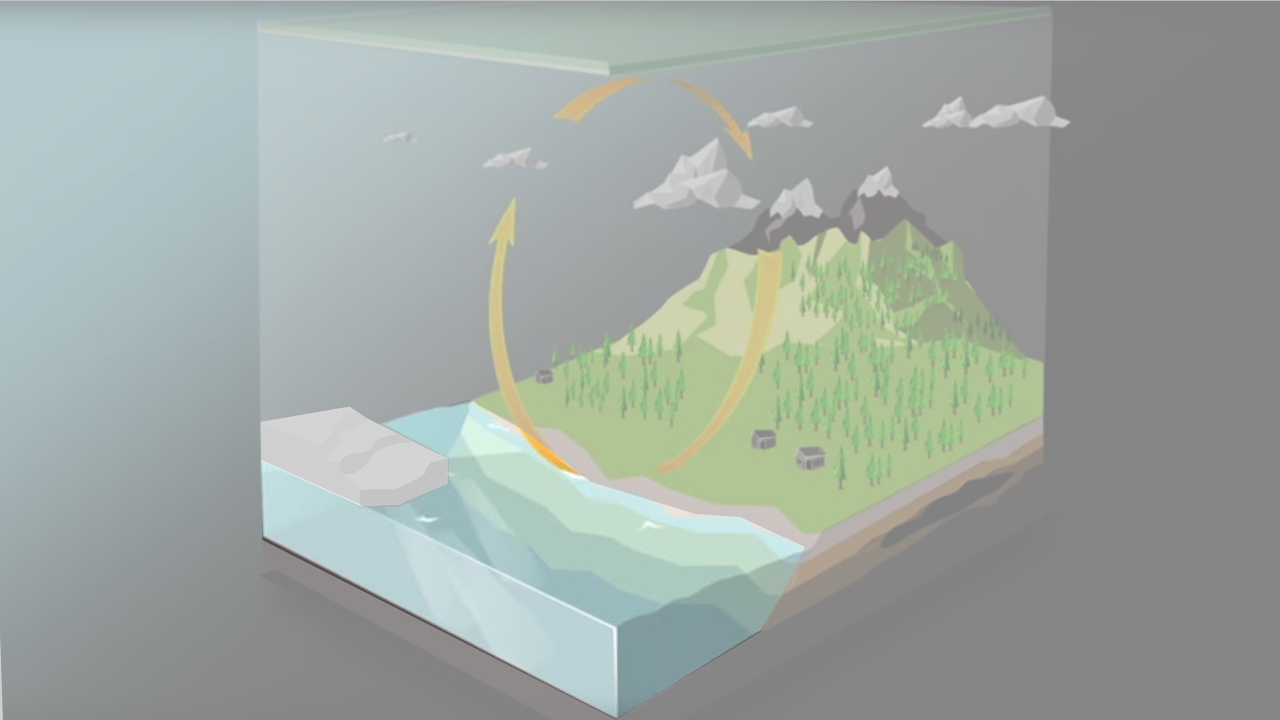
\includegraphics{bilder/WMO_Cycles_water.png}
		\caption{Etwa 2/3 der Erdoberfläche sind von Wasser bedeckt, somit ist die Hydrosphäre allein durch die Masse ein wichtiger Faktor des Klimasystems.}
	\end{figure}

	\note{
	\begin{itemize}
		\item[] Etwa 2/3 der Erdoberfläche sind von Wasser bedeckt, somit ist die Hydrosphäre allein durch die Masse ein wichtiger Faktor des Klimasystems.
		\item[] Daher widmen wir uns zuerst den Wassermassen.
		% Aufteilung von https://www.lenntech.de/faq-wasser-menge.htm, aber auch Wetzel, Robert G. 1983 in "Periphyton of freshwater ecosystems"
    \item[] Der Großteil der Wassermassen ist Salzwasser 97\,\%.
    \item[] Süßwasser (Flüsse und Seen) bildet nur weniger als 1\,\% des globalen Wassers.
    \item[] Eismassen machen ca. 2\,\% des Wassers aus und binden den größten Teil des Süßwassers, da das Salz bei der Eisbildung im Wasser gelößt bleibt.
    \item[] Eis betrachten wir später.
	\end{itemize}
	}
\end{frame}


\begin{frame}
	\frametitle{Eigenschaften des Wassers} % M.Latif Klimawandel und Klimadynamik S. 23
	\begin{itemize}
		\item Wasser ist ein Dipol-Molekül \textcolor{blue}{H$_2$O}
		\begin{itemize}
			\item[$\rightarrow$] Kann wirksam Infrarotstrahlung absorbieren
			\item[$\rightarrow$] Kann viel Wärme aufnehmen bevor es verdampft $\rightarrow$ "Trägheit"
		\end{itemize}

		%Allgemein liegt die größte Dichte des Wassers bei 4 Grad
		\item<2-> Größte Dichte von reinem Wasser bei \SI{4}{\degreeCelsius}
		\begin{itemize}
			\item<2->[$\rightarrow$] Eis schwimmt auf Wasser
		\end{itemize}
		% Im besonderen Fall des Salzwassers liegt die größte Dichte jedoch bei -3.8 Grad
		\item<3->Größte Dichte von Salzwasser bei \SI{-3,8}{\degreeCelsius}
		\begin{itemize}
			\item<3-> [] Bei der Eisbildung wird verbleibt das Salz gelößt im Wasser
			\item<3-> [$\rightarrow$] Wasser kann kälter werden als Eis und sinkt in die tieferen Schichten des Ozeans
			\item<3-> [$\rightarrow$] Wärmeres, weniger dichtes Wasser steigt auf
			\item<3-> [] \textbf{\textcolor{blue}{Konvektion}} in den Polarregionen
			\item<3-> [$\rightarrow$] Kohlenstoffsenken
		\end{itemize}
	\end{itemize}

	\note{
		\begin{itemize}
      \item[] erst die Slide vorstellen
			\item[] Das Phänomen Konvektion ist nicht auf Wasser beschränkt. Gibt es auch in der Luft oder wird durch Pumpen erzeugt.
			\item[] die Konvektion ist durch die temperaturbedingte Dichte und den Salzgehalt möglich
			\item[] daher auch unter dem Namen \textit{thermohaline Konvektion} (thermo - Temperatur, halin - Salz) bekannt
		\end{itemize}
	}

% TODO: evtl. Abbildung der Konvektion: Abgabe von Wärme bei Aufnahme von atmosphärischen Gasen, die dann in die Tiefsee gelangen und dort gespeichert werden

%TODO: Erklärung von Senken
\end{frame}

\begin{frame}
	\frametitle{Wasserdynamik} %M. Latif Klimawandel und Klimadynamik S.24
	\begin{figure}
    \centering
    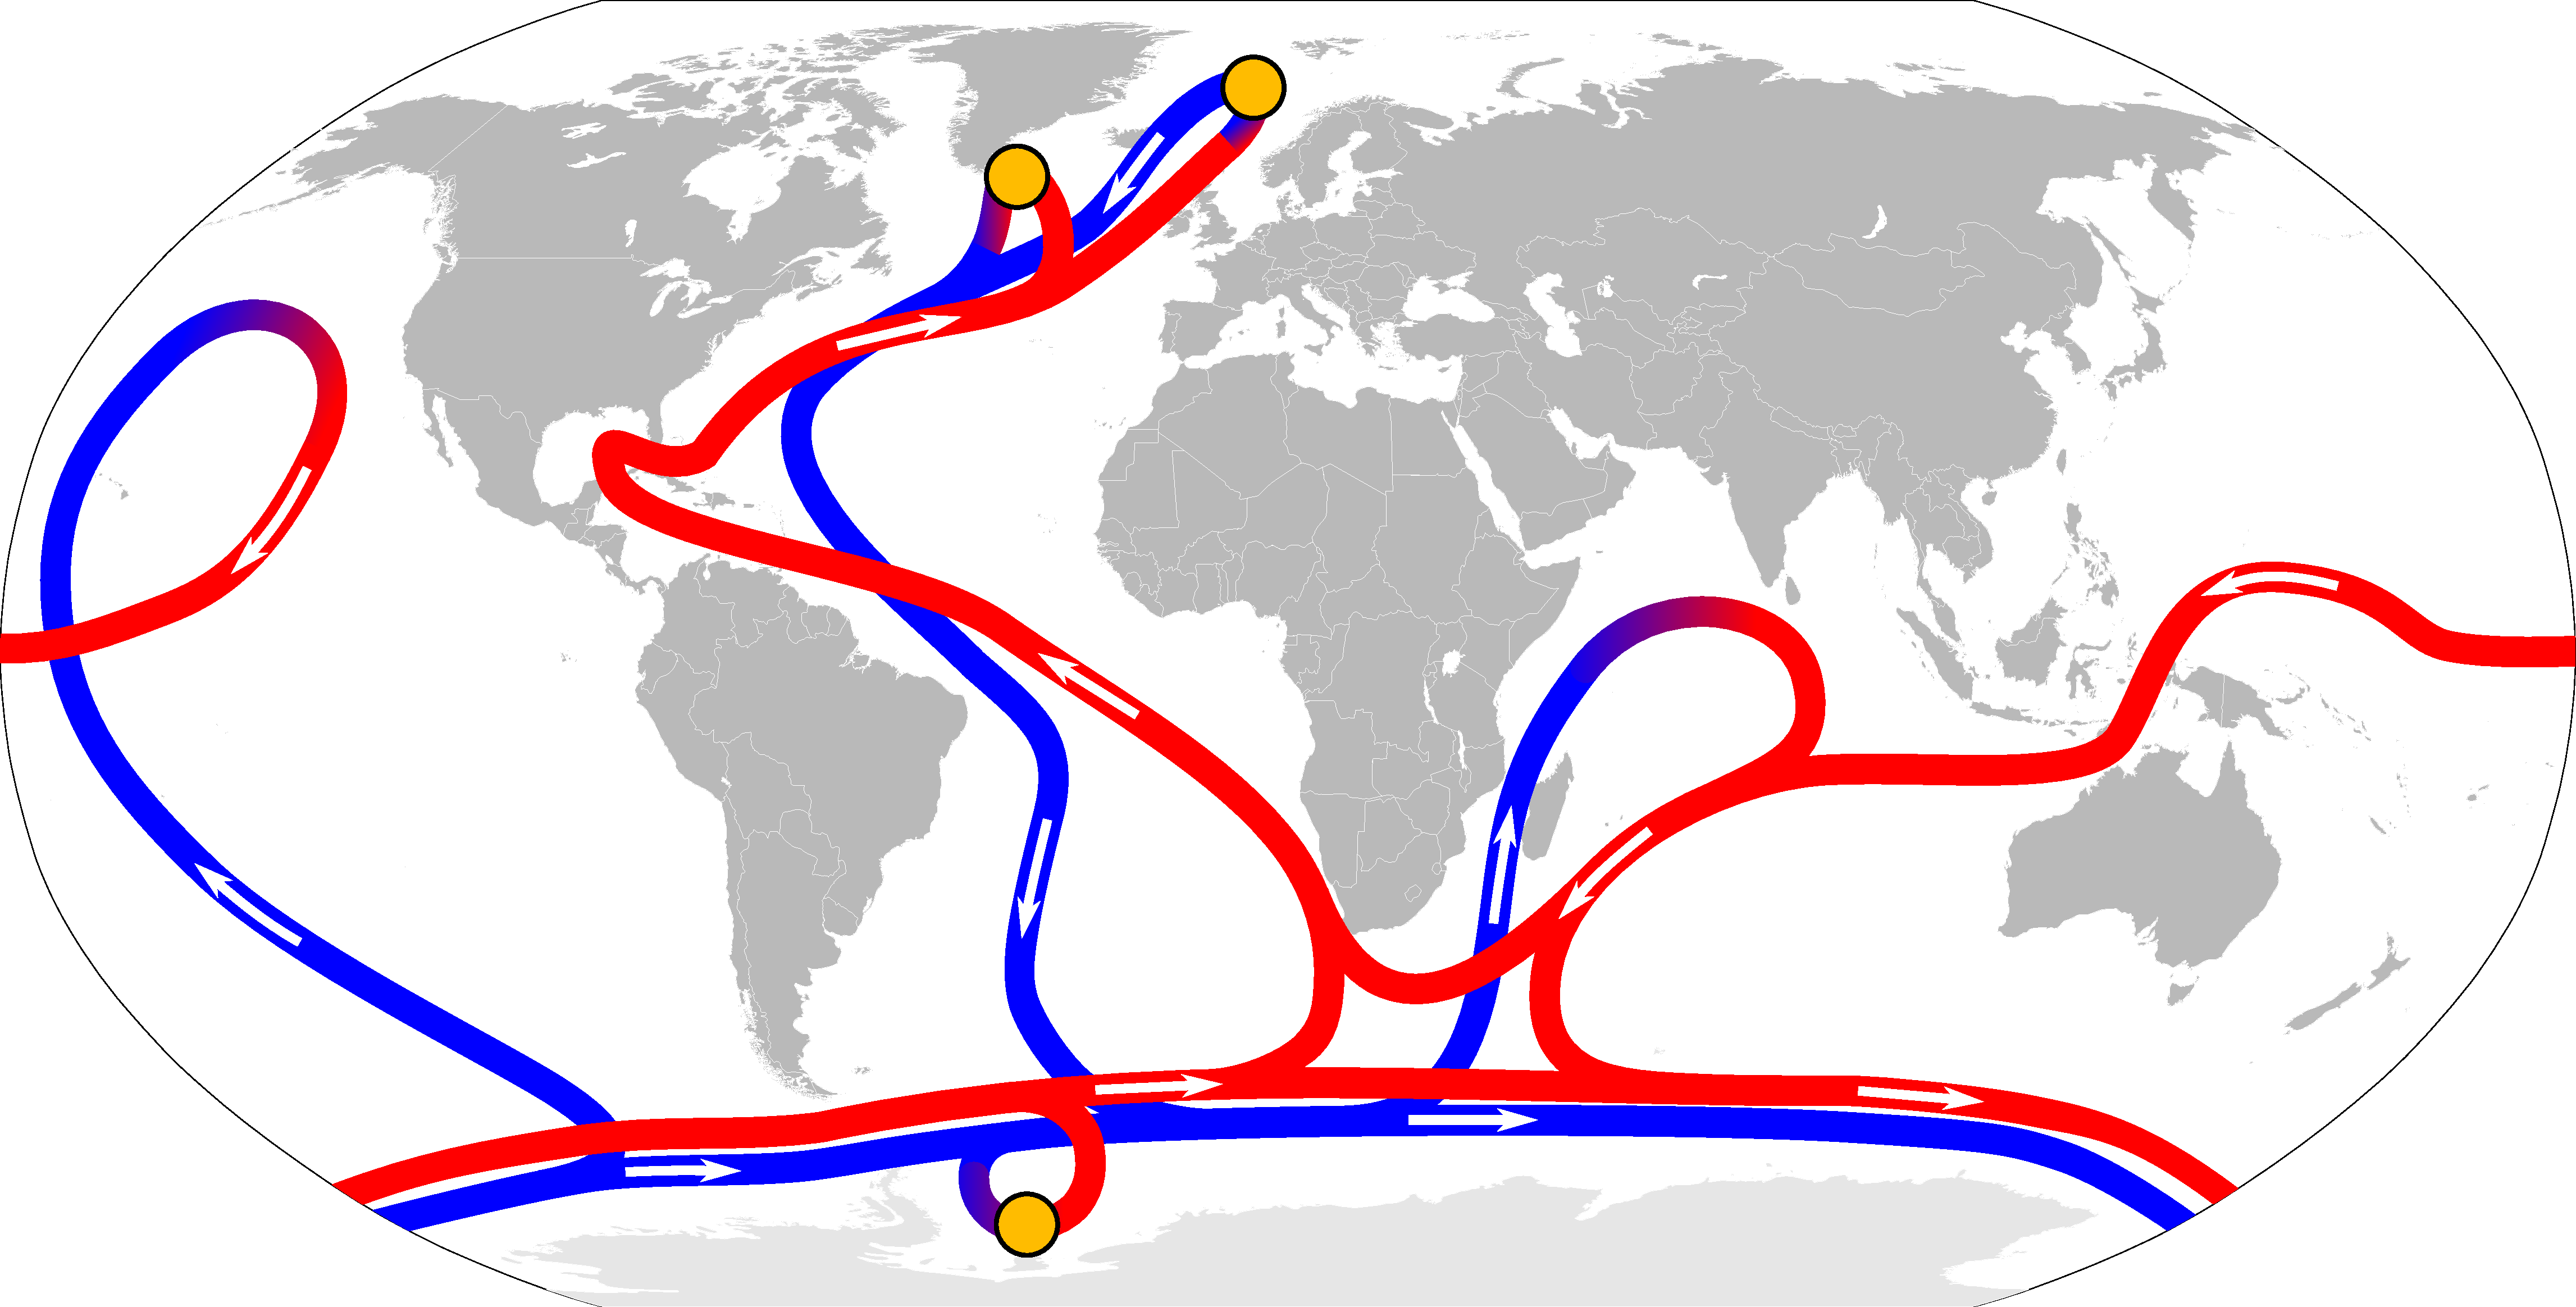
\includegraphics[width=.9\linewidth]{bilder/Thermohaline_Circulation.pdf}
    \caption{Termohaline Zirkulation, Quelle: nach Robert Simmon, NASA}
  \end{figure}

	\note{
		\begin{itemize}
			\item[] Die großen Wassermassen der Ozeane haben eine bestimmte Strömung, z.B. Golfstrom von der Arktis über die Küste Mexikos bis an die Antarktis.
			\item[] Die Stömung ergibt sich vorallem durch die Erdrotation (Corioliskraft).
			\item[] Die oberflächliche Strömung der oberen 100 Meter entsteht durch Wind (und darauf resultierende Reibung) und die Form der Meeresbecken.
			\item[] Die Tiefenströmung wird durch die Konvektion angetrieben. Die Dichte des Wassers spielt dabei eine entschiedende Rolle, da dichteres Wasser nach unten sinkt und leichteres empor steigt.
			\item[] Warme Temperaturen führen zum aufwärmen des Oberflächenwassers und damit zu einer geringeren Dichte.
			\item[] Dadurch werden Oberflächenwasser und Tiefenwasser stark getrennt - und somit strömen die Wassermassen mit unterschiedlicher Geschwindigkeit.
      \item[] Unterscheidung zwischen zwei Zirkulationen
      \begin{itemize}
        \item[Windgetrieben] Oberflächenströmung der Ozeane durch Reibung, Erdrotation (Corioliskraft) und Form der Meeresbecken, eher horizontal
        \item[Dichtegetrieben] Erwärmung, Abkühlung, und Änderung des Salzgehaltes (durch Eisbildung, Verdunstung oder Niederschlag) haben Einfluss auf die Dichte des Wassers, wodurch die Wassermassen zirkulieren, eher vertikal
      \end{itemize}
		\end{itemize}
	}

\end{frame}


\begin{frame}
	\frametitle{Wirkung des Wassers auf das Klima}
	\begin{itemize}
	\item Ca. 70\,\% der Erdoberfläche ist mit Wasser bedeckt
	\item [$\rightarrow$] Die \textit{Trägheit} des Wassers ist ein entscheidender Faktor für die Trägheit des Klimas und der Klimaänderungen % M.Latif Klimawandel und Klimadynamik S. 23
	\item Kohlenstoffsenken in der Tiefsee können durch erwärmen der Ozeane \textit{irgendwann} freigesetzt werden
	\item[$\rightarrow$] massiver Anstieg des atmosphärischen CO$_2$ $\rightarrow$ Verstärkung des Treibhauseffekts
	\item Positive Verstärkung von CO$_2$ und Wasserdampf: eine wärmere Atmosphäre kann mehr Wasserdampf (und CO$_2$) aufnehmen
	\end{itemize}
\end{frame}

\begin{frame}
	\frametitle{Trägheit des Klimas}
	\begin{figure}
		\centering
		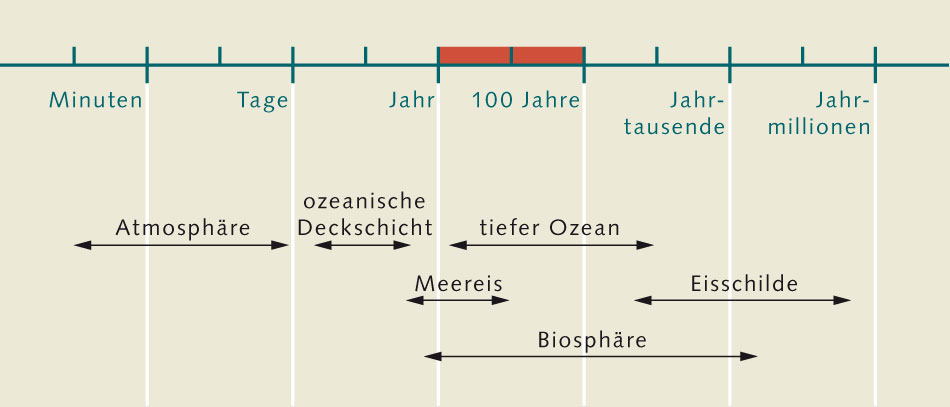
\includegraphics[width=0.8\linewidth]{bilder/zeitskala-klimasystem_world_ocean_review.jpg}
		\caption{Zeitskalen im Klimasystem, Quelle: maribus nach Meinecke und Latif, 1995}
		\label{fig:traegheit}
	\end{figure}

  \begin{itemize}
    \item[$\rightarrow$] Verzögertes Feedback bis zu einem klimawirksamen Ereignis.
    \item[$\rightarrow$] Besonders die Ozeane und Eisschilde benötigen eine sehr lange Zeit, um sich geänderten klimatischen Bedingungen anzupassen.
  \end{itemize}

	\note{
		\begin{itemize}
			\item[] Trägheit des Wassers ist entscheident.
			\item[] Die Wassermassen sind in dieser Abbildung stark vertreten.
			\item[] Die untere Atmosphäre passt sich innerhalb weniger Stunden den Bedingungen der Erdoberfläche an (Temeperatur, Gase, etc.)
			\item[] Die Wassermassen reagieren sehr unterschiedlich.
			\item[] Flüsse, Seen und Oberflächenwasser wärmen sich dabei deutlich schneller auf als die tieferen Ozeanschichten. (Das kennt man vielleicht aus Bade- oder Bergseen - die oberen 50 cm sind angenehm warm und darunter liegt deutlich kälteres Wasser)
			\item[] Besonders unterschiedlich schnell reagiert die Biosphäre.
      \begin{itemize}
        \item[] Graslandschaften können schnell austrocken
        \item[] Wälder dagegen verändern sich über Jahrtausende hinweg.
        \item[] Die Vegetation bestimmt in vielen Fällen auch die Ansiedlung von Lebewesen.
        \item[] Die Änderung der Vegetation kann das Ende des Lebenraums einiger Lebewesen bedeuten, aber auch neue Ansiedluneg bedingen.
      \end{itemize}
			\item[] Eine besonders lange Reaktionszeit haben die Eisschilde der Erde. Auf die Eismassen gehen wir als nächstes ein.
		\end{itemize}
	}
\end{frame}

\begin{frame}
	\frametitle{Kryosphäre - Eismassen}

	\begin{figure}
		\centering
		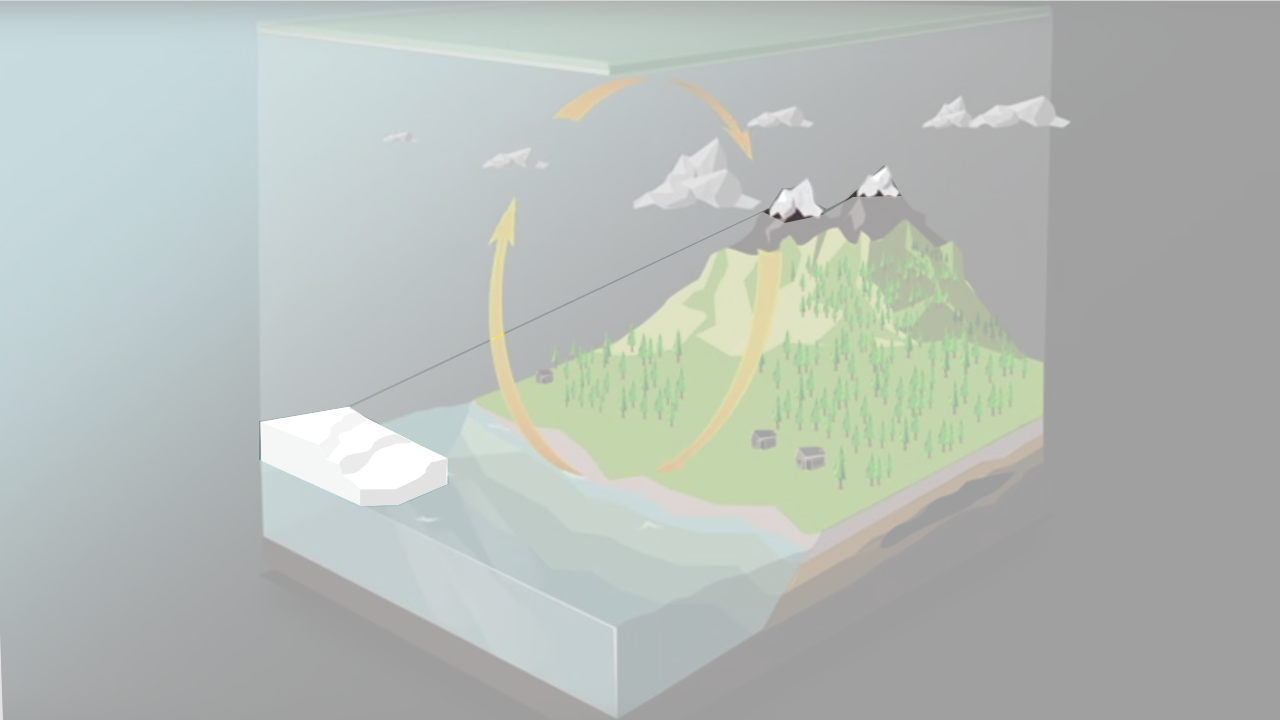
\includegraphics{bilder/WMO_Cycles_ice.png}
		\caption{Kryosphäre umfasst alle Formen und Schnee und Eis}
	\end{figure}
	\note{
		\begin{itemize}
			\item[] Eismassen stellen nach den Ozeanen die zweitgrößte Komponente des Klimasystems dar.
			\item[] das liegt an der Wärmekapazität von Wasser und seinem Volumen
      \begin{itemize}
        \item[] Wasser: \SI{4,18}{kJ \per kg \per K} bei \SI{20}{°C}
        \item[] Gestein etwa: \SIrange{0,7}{1}{kJ \per kg \per K}
      \end{itemize}
      \item[] ca. 2\,\% des Wassers ist in fester Form in Gletschern und an den Polkappen dauerhaft gebunden.
  %		\item  inländische Eisflächen speichern ca. 75\% des globalen Süßwassers
  		\item[] Eis reflektiert die ankommende Sonnenstrahlung zu großen Teilen
  		$\rightarrow$ \textbf{\textcolor{blue}{Albedo-Effekt}}\\

  		\item[] Je weniger Eismassen, desto weniger Strahlung wird reflektiert und bleibt in der Atmosphäre $\rightarrow$ Verstärkung des Treibhauseffekts

  		\item[] Durch Rußablagerungen auf den Eismassen wird mehr Sonnenstrahlung absorbiert ("Black Carbon")
  		 $\rightarrow$ Schmelzen des Eis und Verringerung des Albedo-Effekts % (Nature Geoscience, 2014; doi: 10.1038/ngeo2180)
		\end{itemize}
	}
\end{frame}


\begin{frame}
	\frametitle{Kryosphäre - Komponenten}
	Die größten Komponenten der Kryosphäre sind:
	\begin{itemize}
		\item Meereis: schwimmende Eismassen, 19-27 Mio. km$^2$
		\item Eisschilde: über Grönland und der Antarktis, 14 Mio. km$^2$
		\item Permafrost: gefrorene Böden, 22,8 Mio. km$^2$
	\end{itemize}

	\glqq Ein einmal eingesetzter Rückzug großer kontinentaler Eisschilde kann selbst nach Stabilisierung der Randbedingungen [(CO$_2$-Emissionen)] über ein Jahrtausend lang anhalten\grqq{} (Latif, 2009 und IPCC, 2001)\\
	%$\rightarrow$ siehe auch: Trägheit des Klimas in Abbildung \ref{fig:traegheit}

	\note{
		\begin{itemize}
			\item[] Meereis flächenmäßig sehr groß, aber Volumen der Eisschilde deutlich größer
			\item[] Eisschilde durchschnittlich 1,7-2 km dick
			\item[] weitere Elemente:
			\item[] Schneebedeckung variiert jahreszeitlich besingt zwischen 2 und 45 Mio. km$^2$
			\item[] Gletscher bilden 'nur' 0.5 Mio. km$^2$
		\end{itemize}
	}
\end{frame}

\begin{frame}
	\frametitle{Meereis} % Bild -> Pexels Andrea Schettino
  \begin{columns}
    \column{.3\linewidth}
    \begin{figure}
      \centering
      \newlength{\imagewidth}
      \settowidth{\imagewidth}{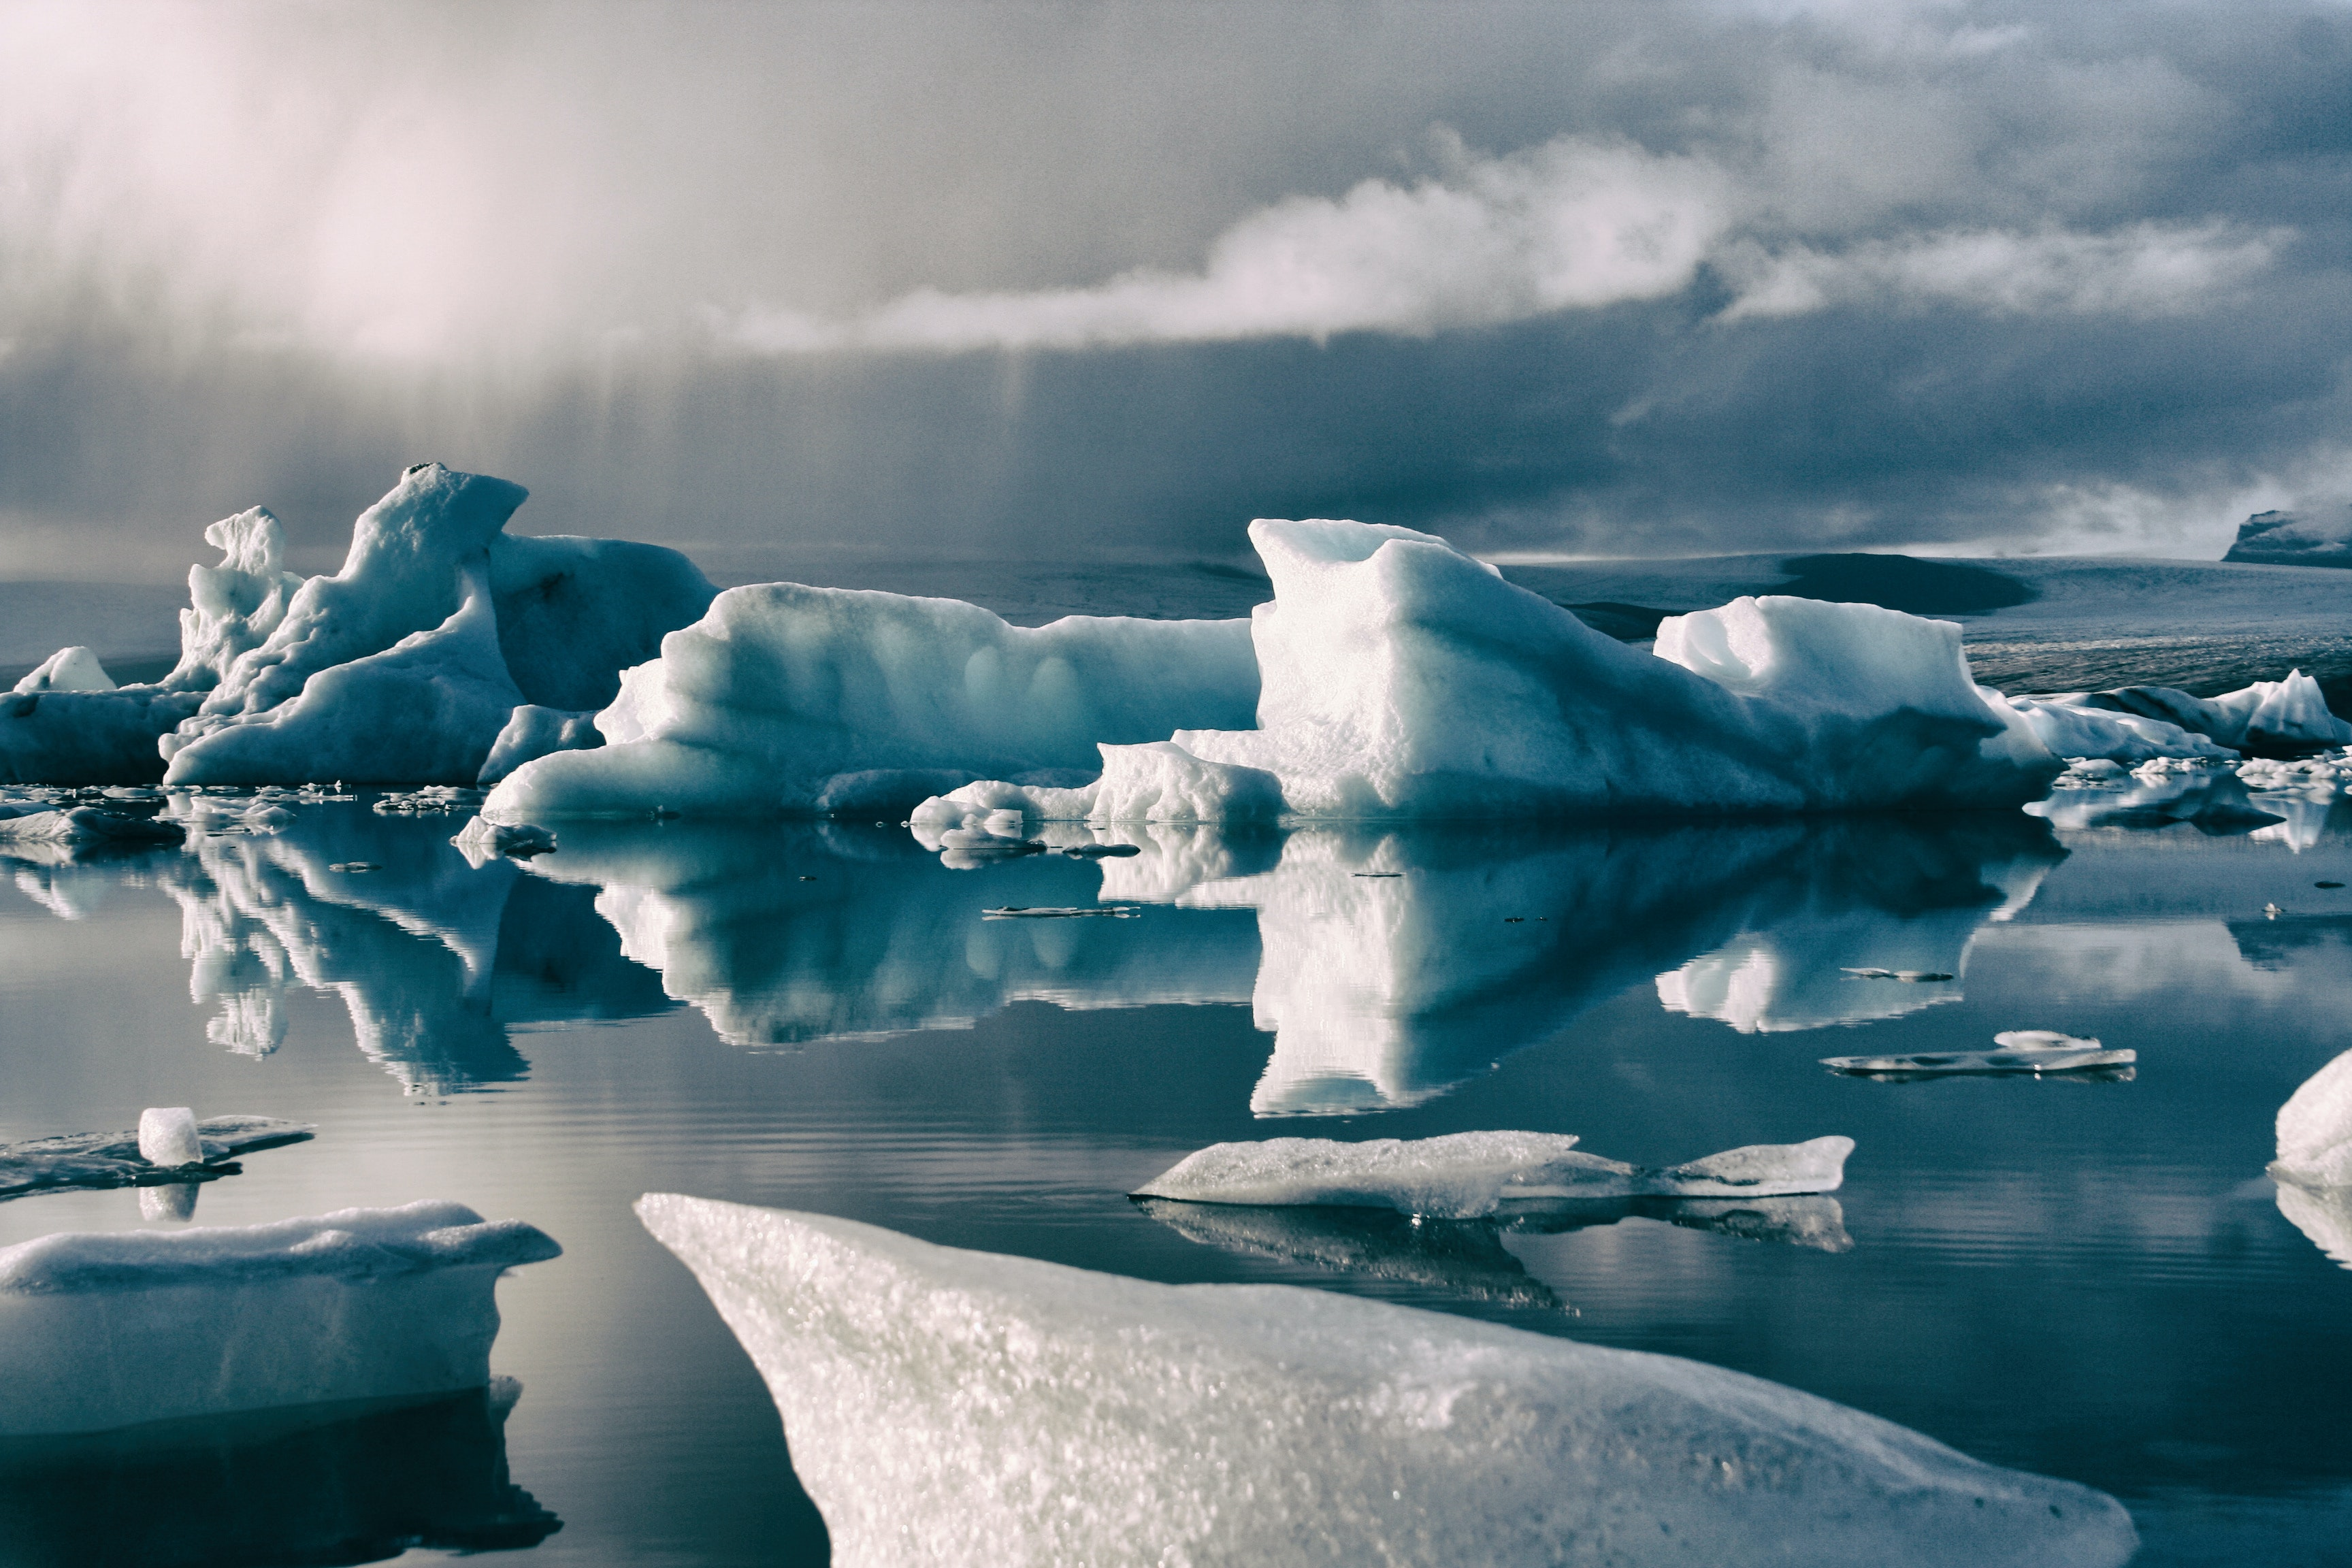
\includegraphics{bilder/ice-formation-in-body-of-water-3923277.jpg}}
      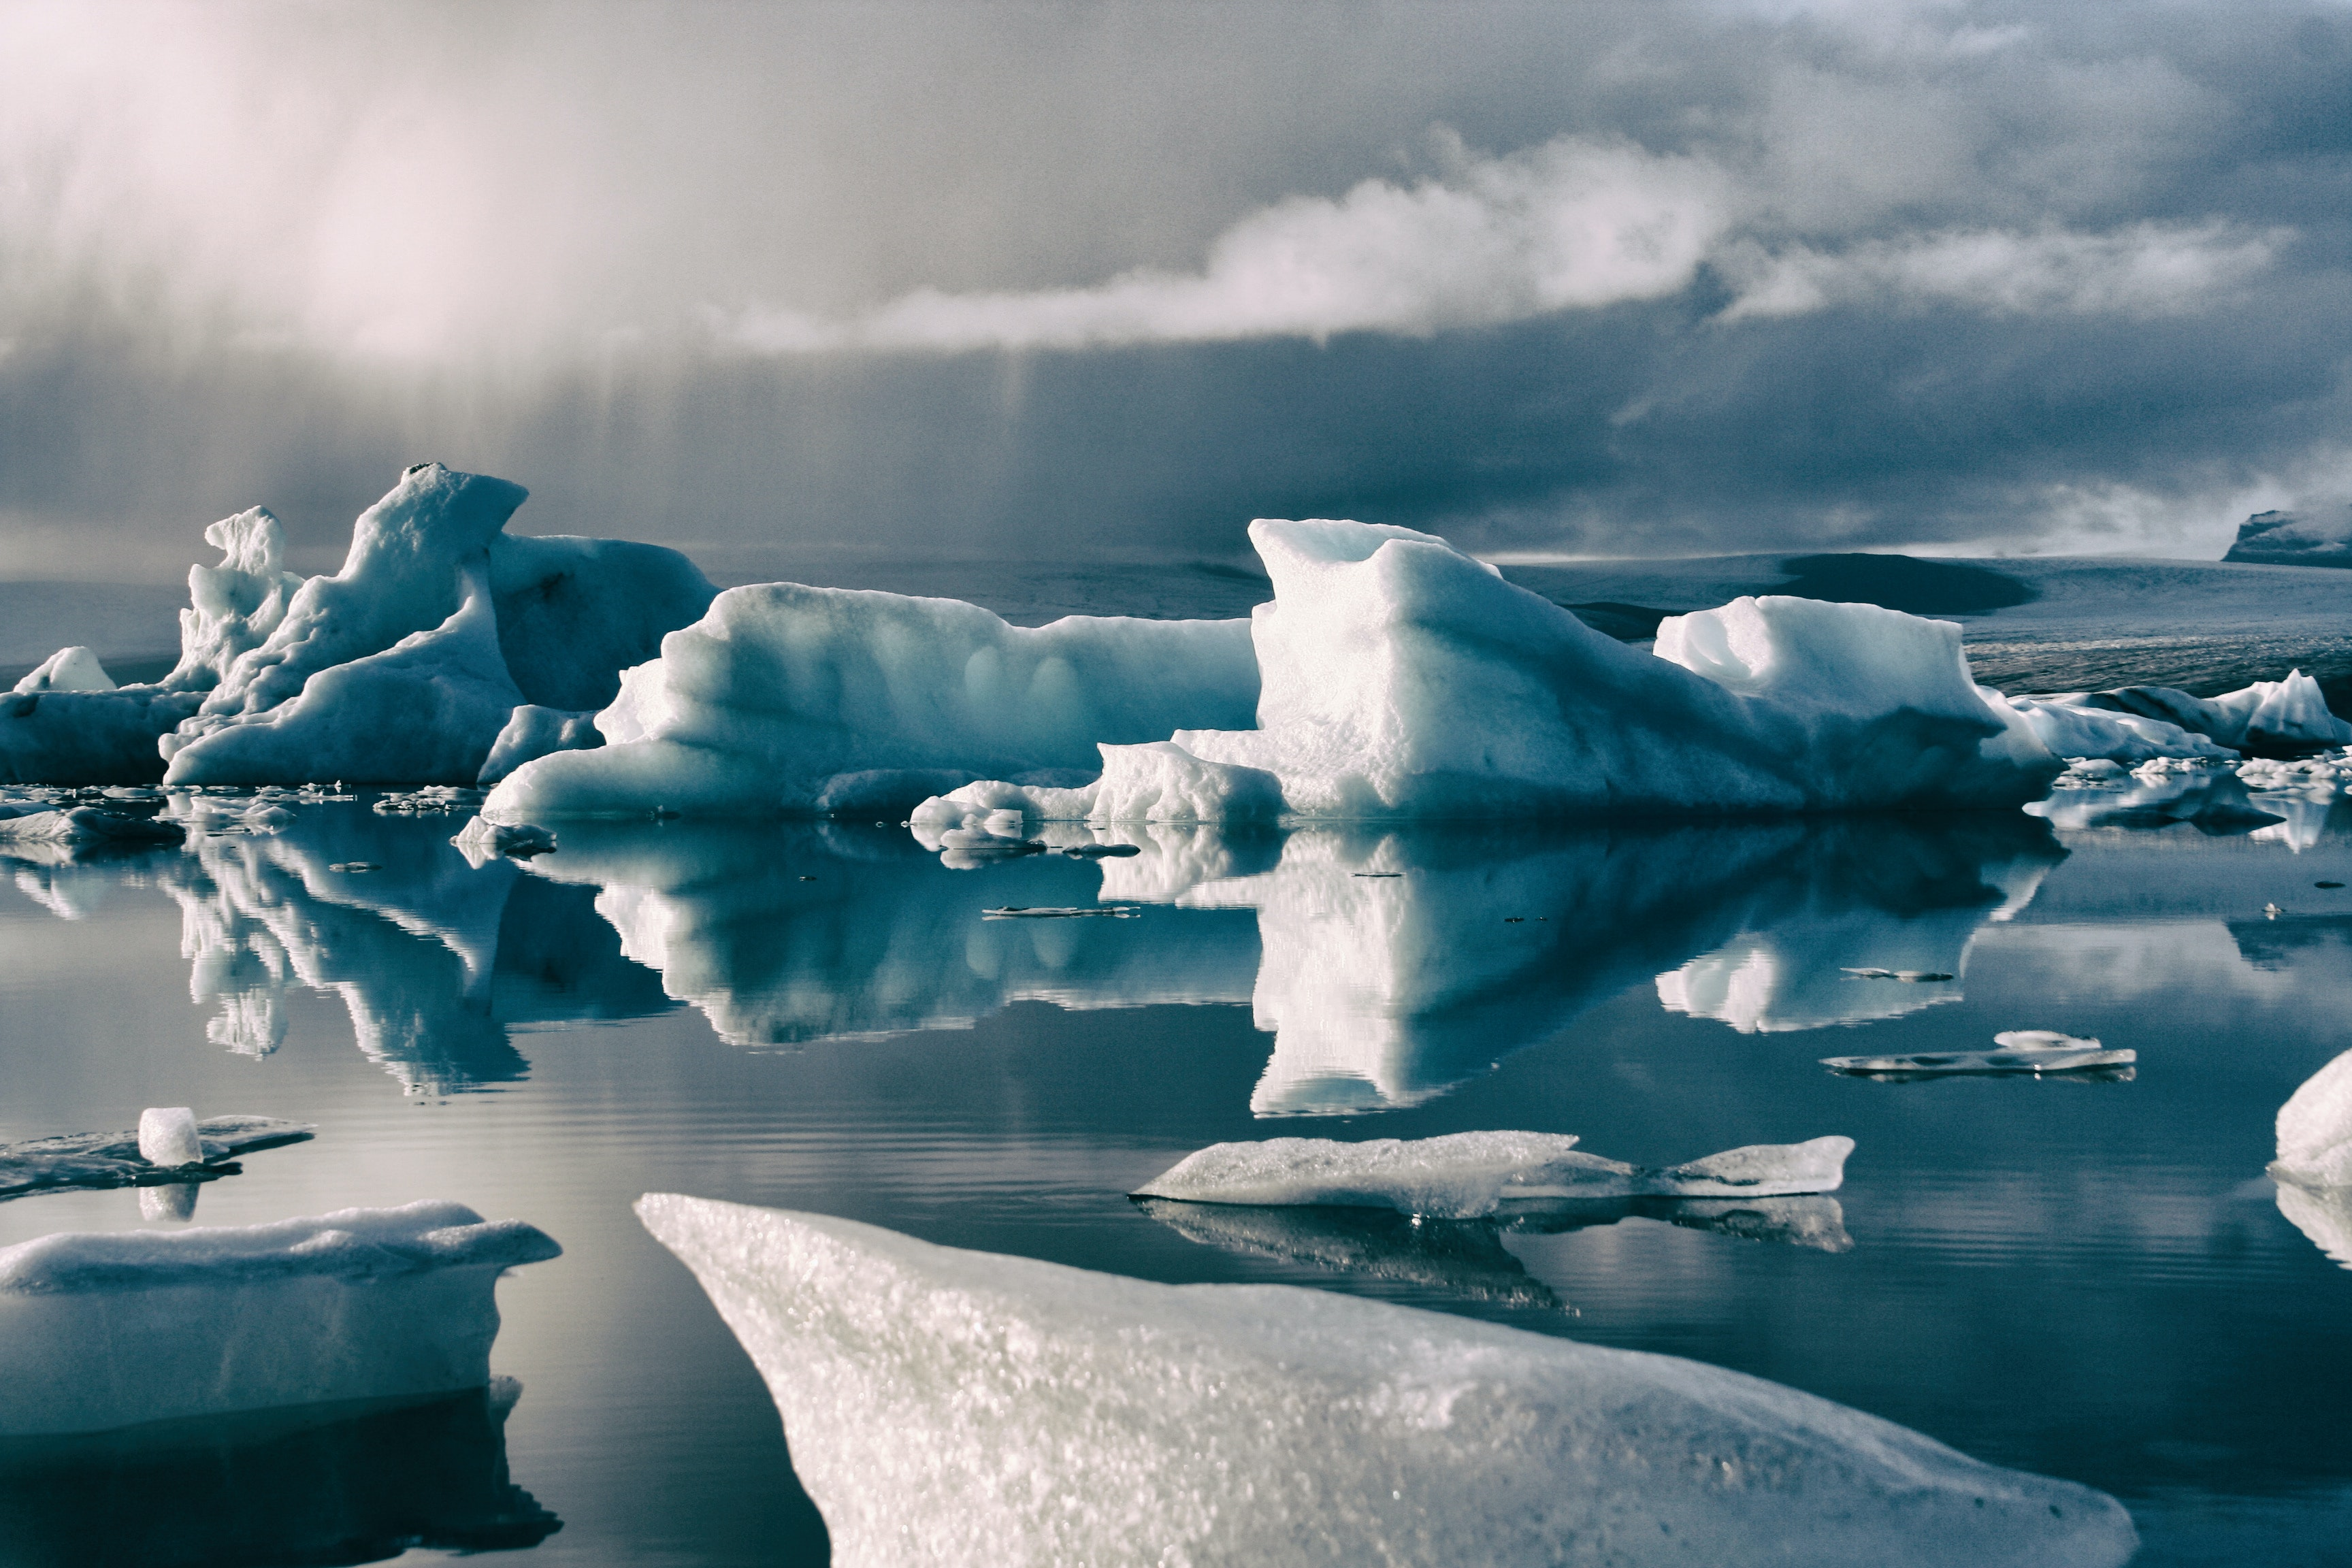
\includegraphics[trim=0 0 0.69\imagewidth{} 0, clip, width = 0.8\linewidth]{bilder/ice-formation-in-body-of-water-3923277.jpg}
      \caption{Quelle: Pexels, Andrea Schettino}
    \end{figure}
    \column{.7\linewidth}
	    \begin{itemize}
		    \item Bildet die Grenze zwischen Ozeanen und Atmosphäre
		    \item Luft über dem Meereis ist deutlich kälter als über dem Ozean
		    \item [$\rightarrow$] Abkühlung der Polarregionen und Verstärkung der atmosphärischen Zirkulation (Winde)
		    \item [$\rightarrow$] Beeinflusst Konvektion: je weniger Eis, desto schwächer die Konvektion, desto schwächer sind (langfristig) ozeanische Strömungen
	   \end{itemize}
   \end{columns}

	\note{
		\begin{itemize}
			\item[] Winde entstehen zum Dichte-/Wärmeausgleich, stärkere Tmeperaturunterschiede führen also zu stärkeren Winden
			\item[] Konvektion beeinflusst vorallem die Tiefseestömungen
			\item[] Weniger Konvektion bedeutet auch weniger Nährstoffe in oberen Schichten der Ozeane
		\end{itemize}
	}
\end{frame}

\begin{frame}
	\frametitle{Eisschilde}
  \begin{columns}
    \column{.3\linewidth}
    \begin{figure}
      \centering
      \settowidth{\imagewidth}{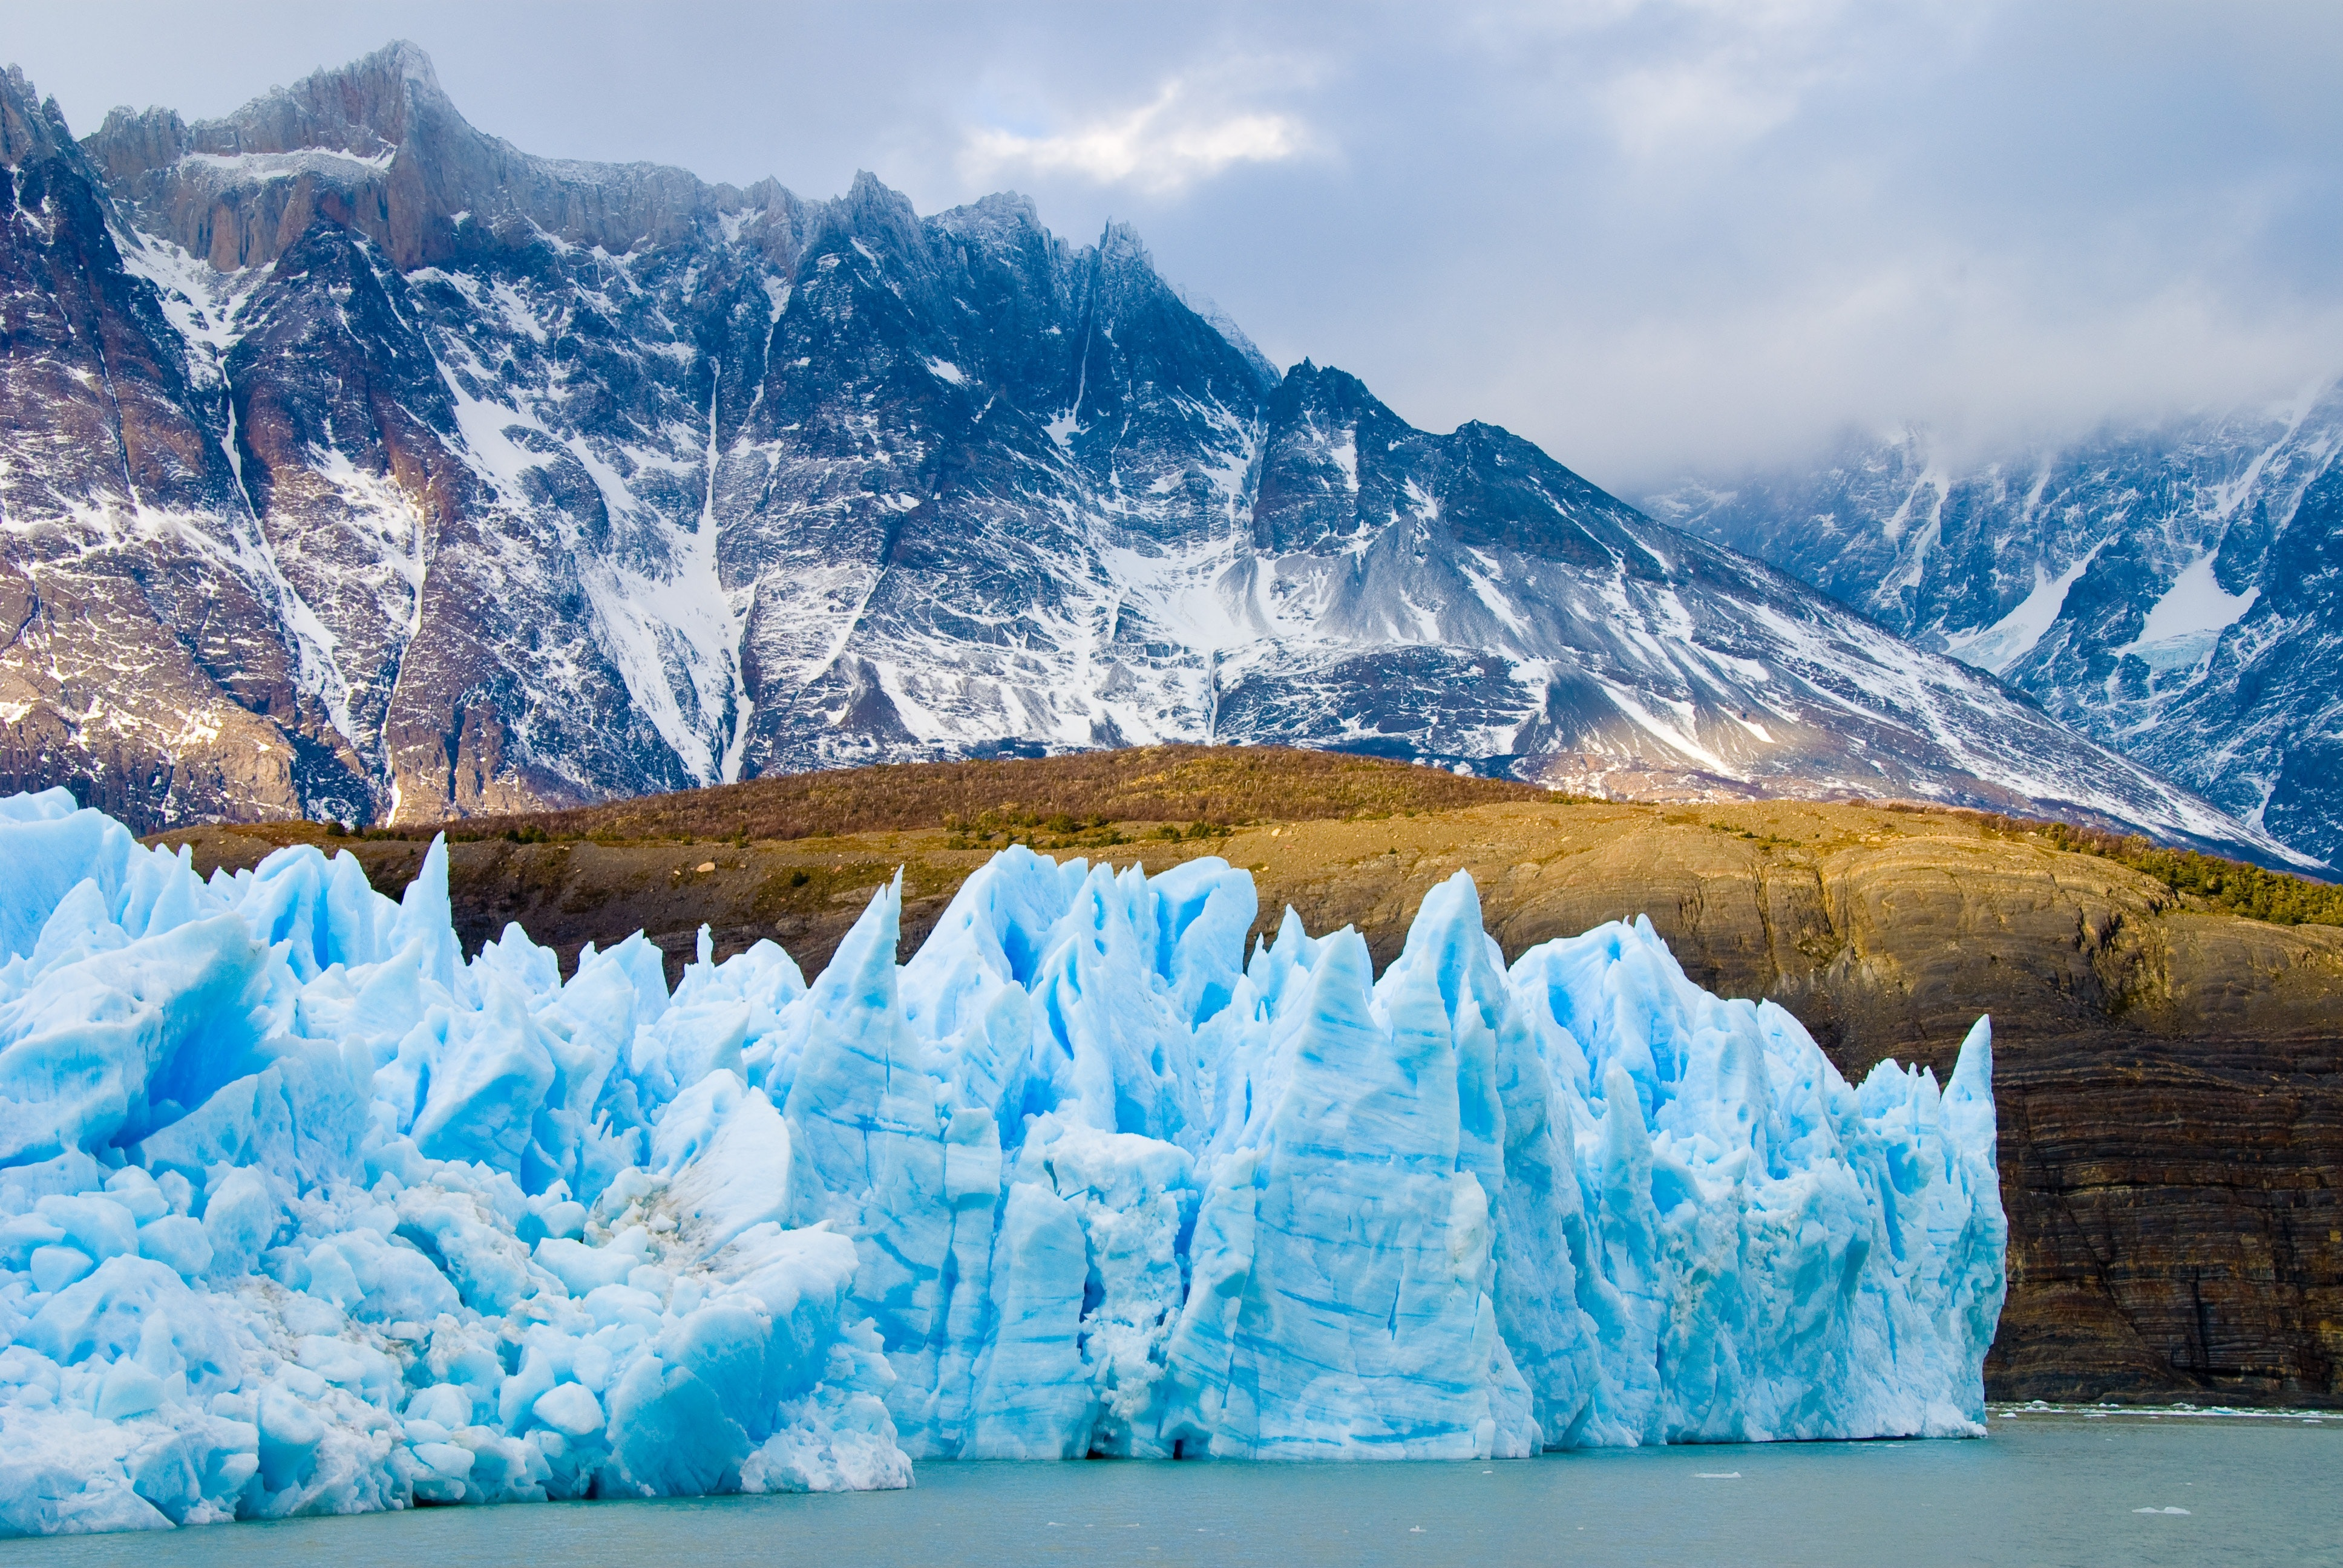
\includegraphics{bilder/panoramic-view-of-landscape-against-sky-255329.jpg}}
      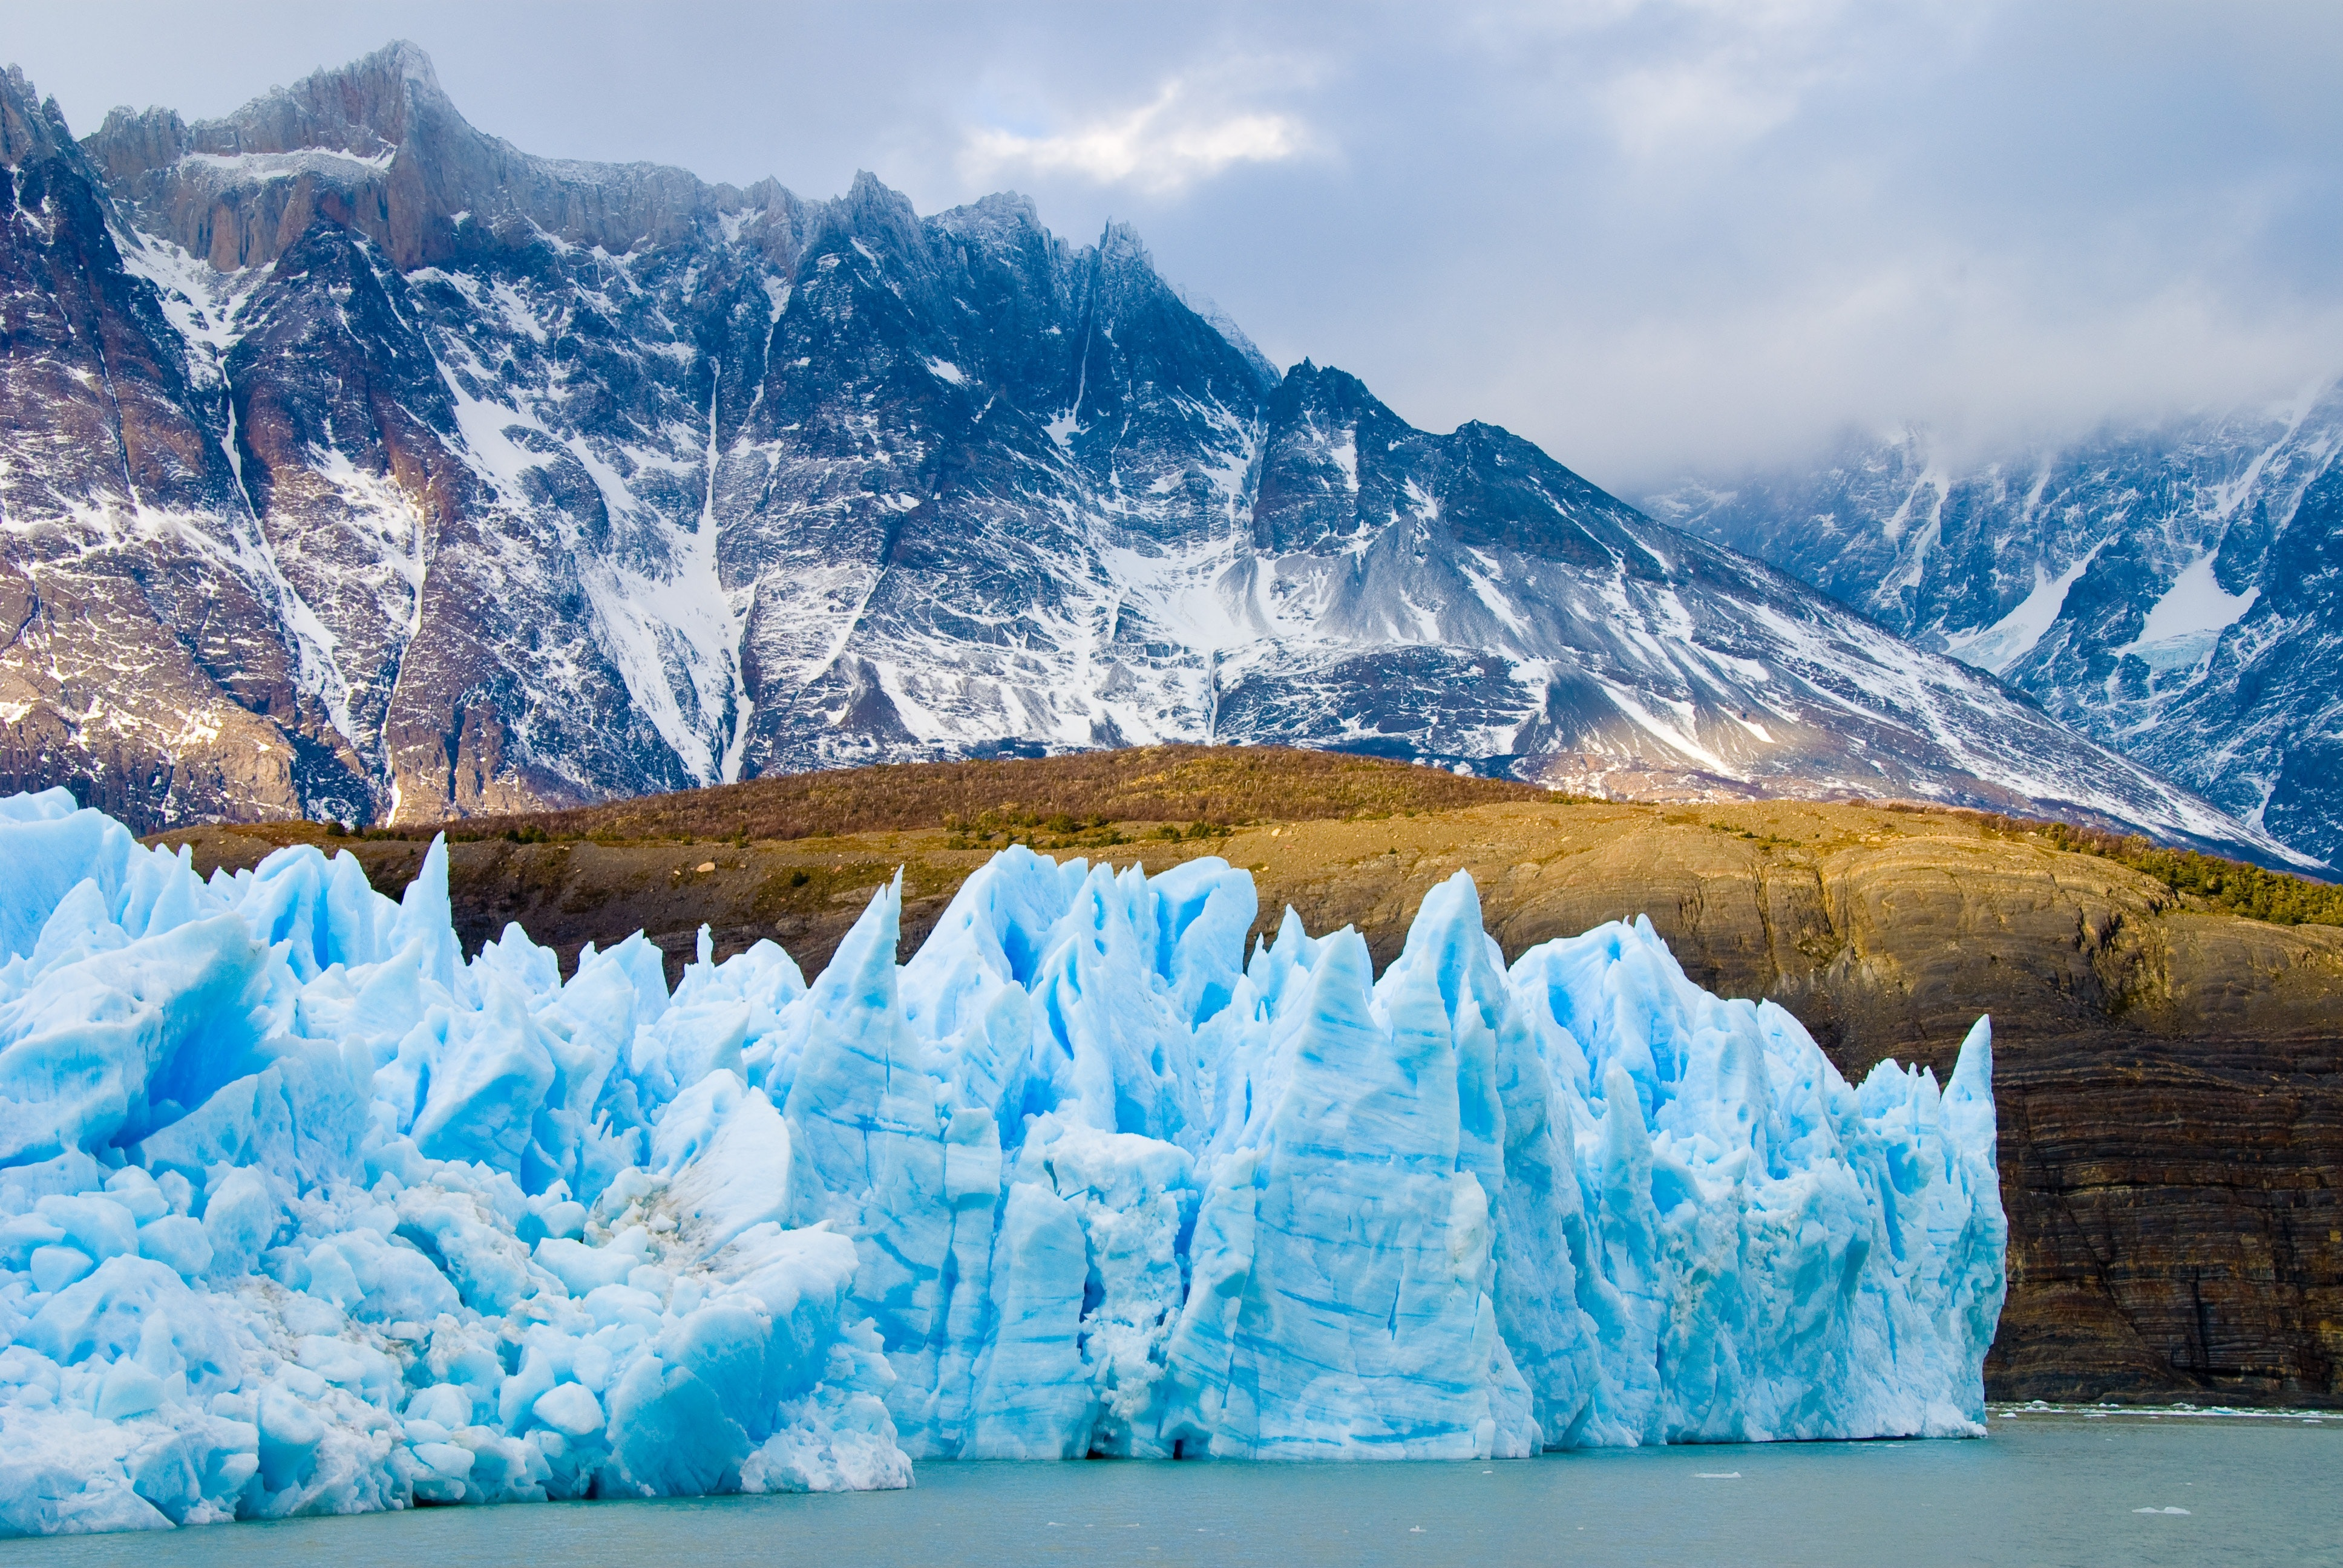
\includegraphics[trim=0 0 0.69\imagewidth{} 0, clip, width = 0.8\linewidth]{bilder/panoramic-view-of-landscape-against-sky-255329.jpg}
      \caption{Quelle: Pexels, Pixabay}
    \end{figure}
    \column{.7\linewidth}
	\begin{itemize}
		\item Volumen: 25 Mio. km$^3$ (Antarktis) + 3 Mio. km$^3$ (Grönland)
		\item Masse ist durch Niederschlag, Lufttemperatur und Strahlung bestimmt
		\item In der Antarktis gibt es Ausläufer des Landeises auf den Ozean hinaus (Schelfeis) $\rightarrow$ 0,7 Mio. km$^3$
%		\item tiefer liegende Schichten der Eisschilde schmelzen durch den Druck auf die Landmassen $\rightarrow$ erzeugt Spannungen im Eis
		\item Eisschilde schmelzen an randnahen Bereichen
		\item Höhere Temperaturen im Nordhalbkugelsommer gefährden das grönländische Eisschild besonders stark
		\item \textbf{Eisschilde haben das größte Potential für einen Anstieg des Meeresspiegels, da sie nicht -- wie das Meereis -- zum Meeresspiegel beitragen}
	\end{itemize}
  \end{columns}

	\note{
		\begin{itemize}
			\item[] Je mehr Schnee und je kälter, desto mehr Eis kann dich bilden
			\item[] Schelfeis zählt nicht zum Meereis, da es fest mit den Eisschilden verbunden ist
			\item[] Schelfeis bildet sich v.a. in Buchten, die von Eisschild umgeben sind
			\item[] Grönland besitzt quasi kein Schelfeis, daher schmilzt in Grönland direkt das Eisschild
			\item[] Der Antarktische Eisschild ist durch das Schelfeis etwas mehr geschützt
			\item[] Ein komplettes Abtauen der Eisschilde kann den Meeresspiegel bis zu 64 Meter ansteigen lassen. $\rightarrow$ sog. Meeresspiegel-äquivalent nach IPCC 2007
		\end{itemize}
	}
\end{frame}

\begin{frame}
	\frametitle{Permafrost}
  \begin{columns}
    \column{.3\linewidth}
    \begin{figure}
      \centering
      \settowidth{\imagewidth}{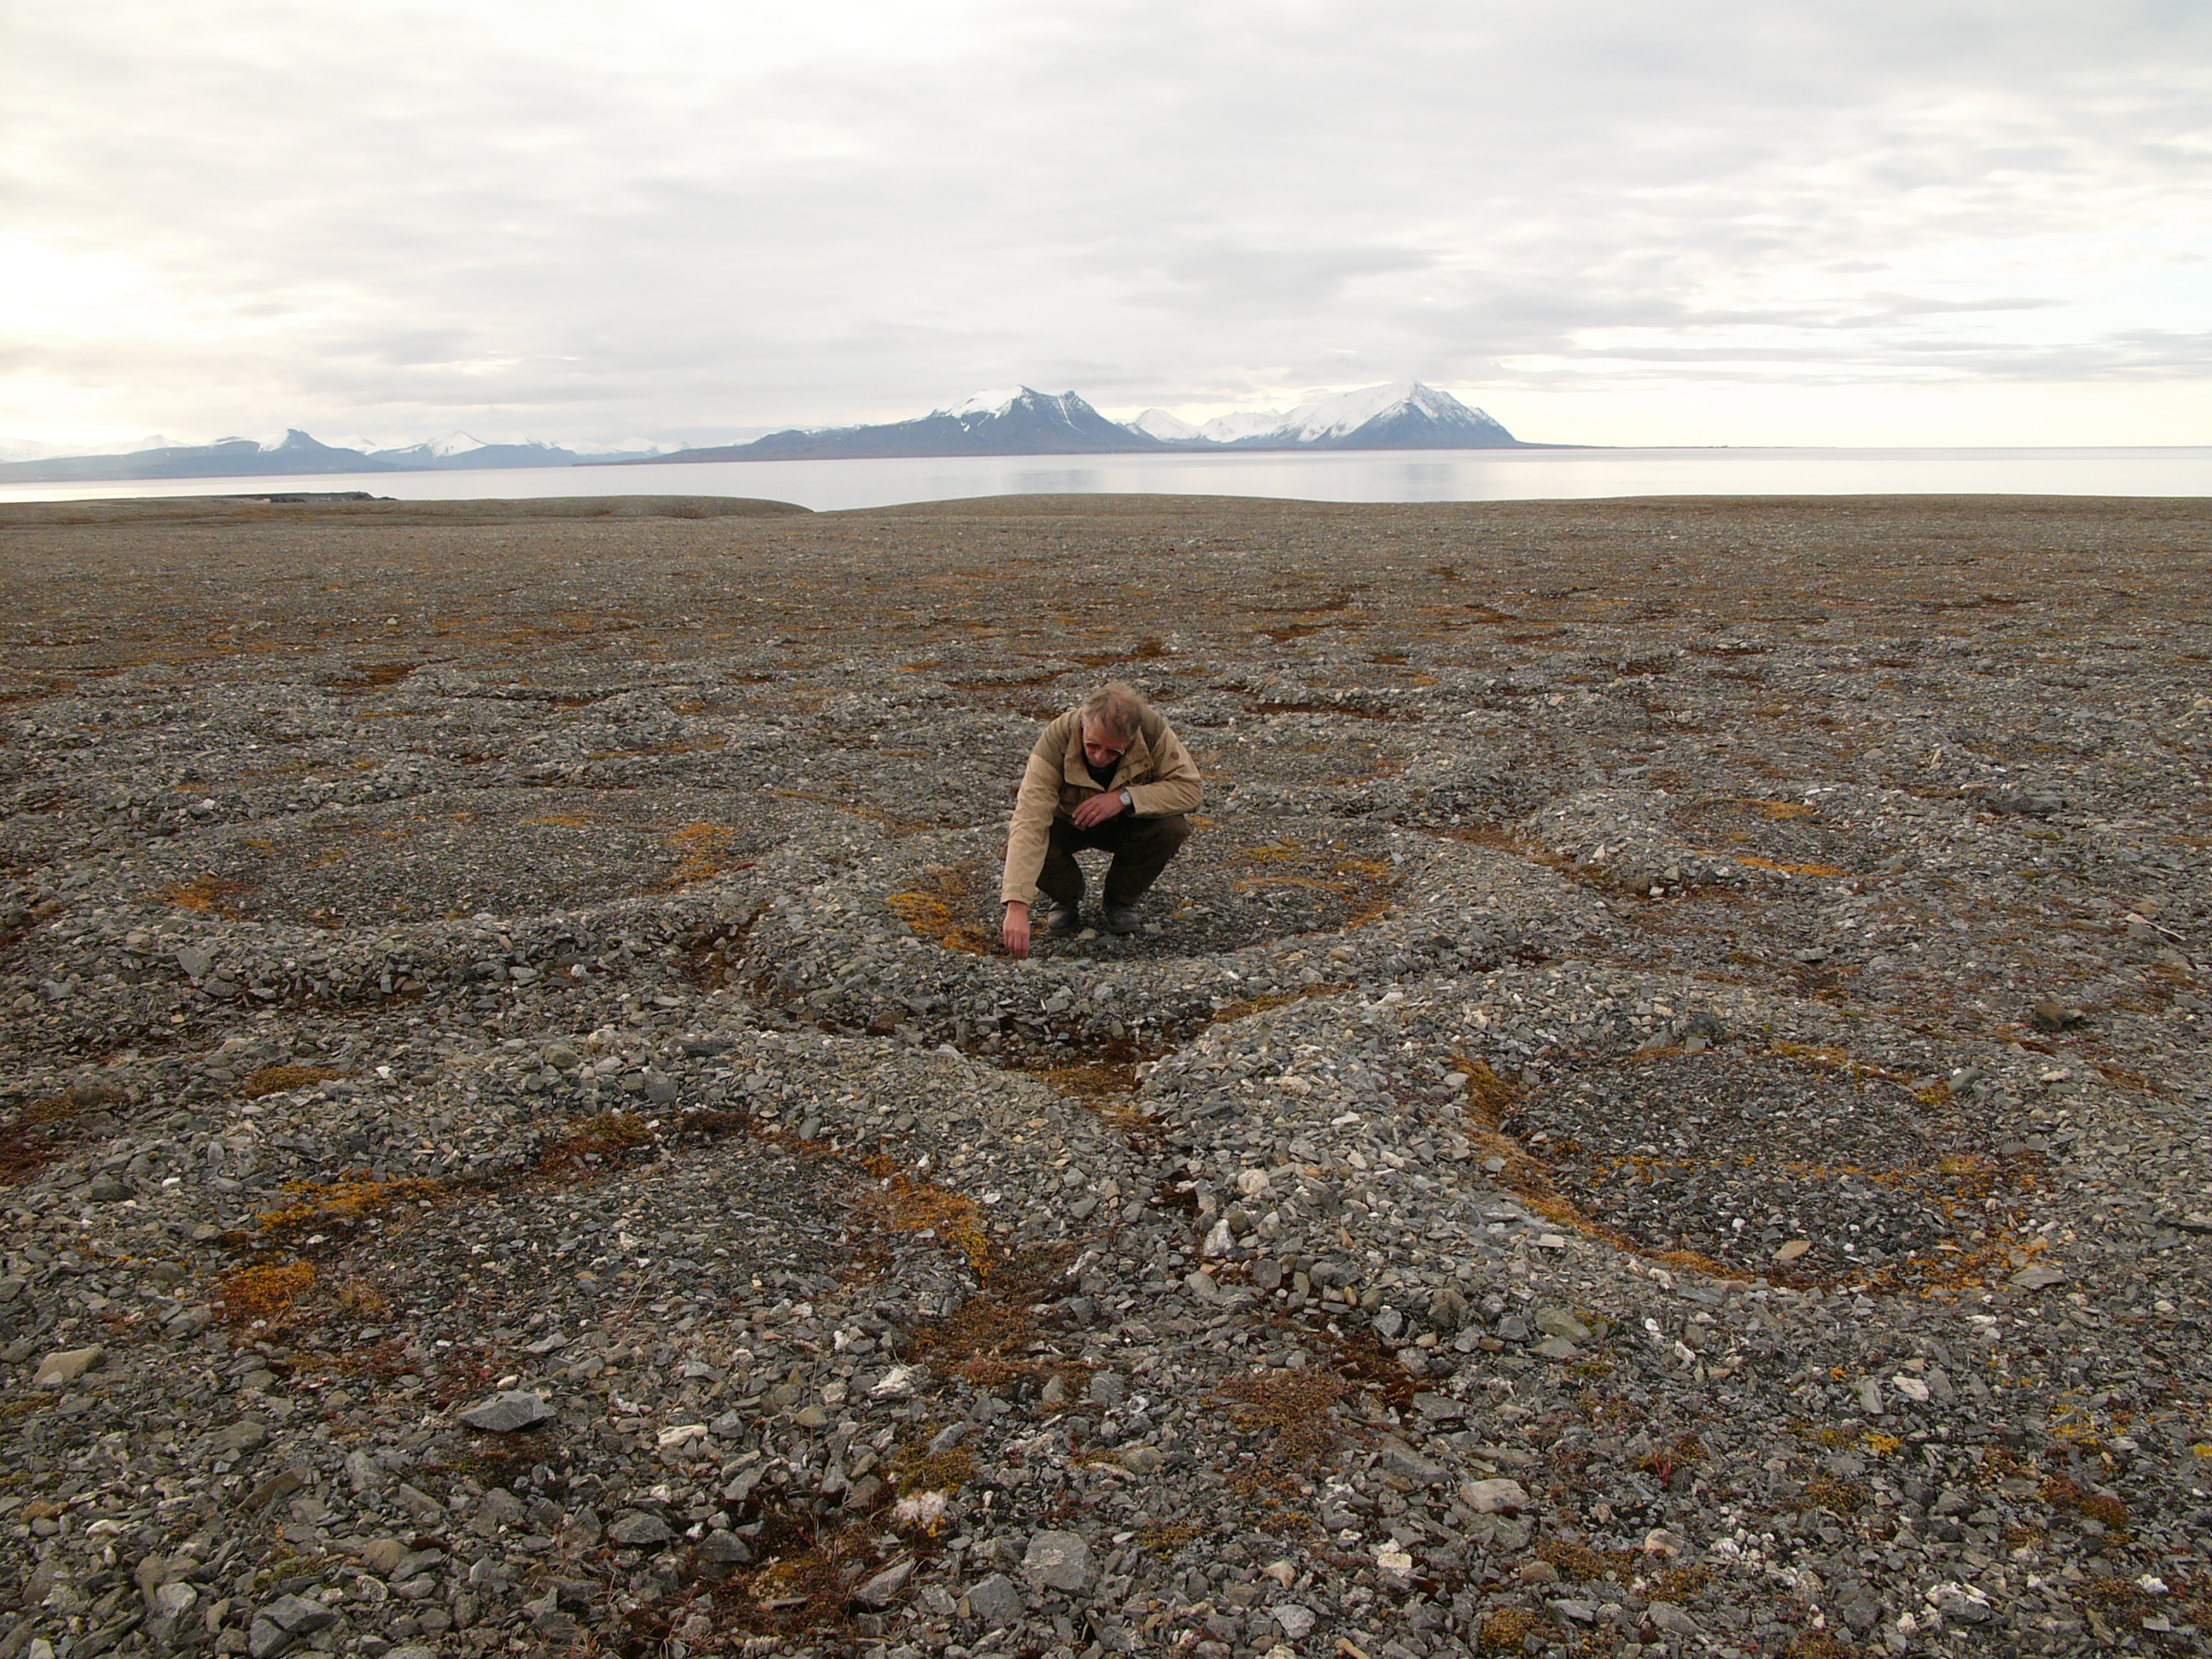
\includegraphics{bilder/Permafrost_stone-rings_hg.jpg}}
      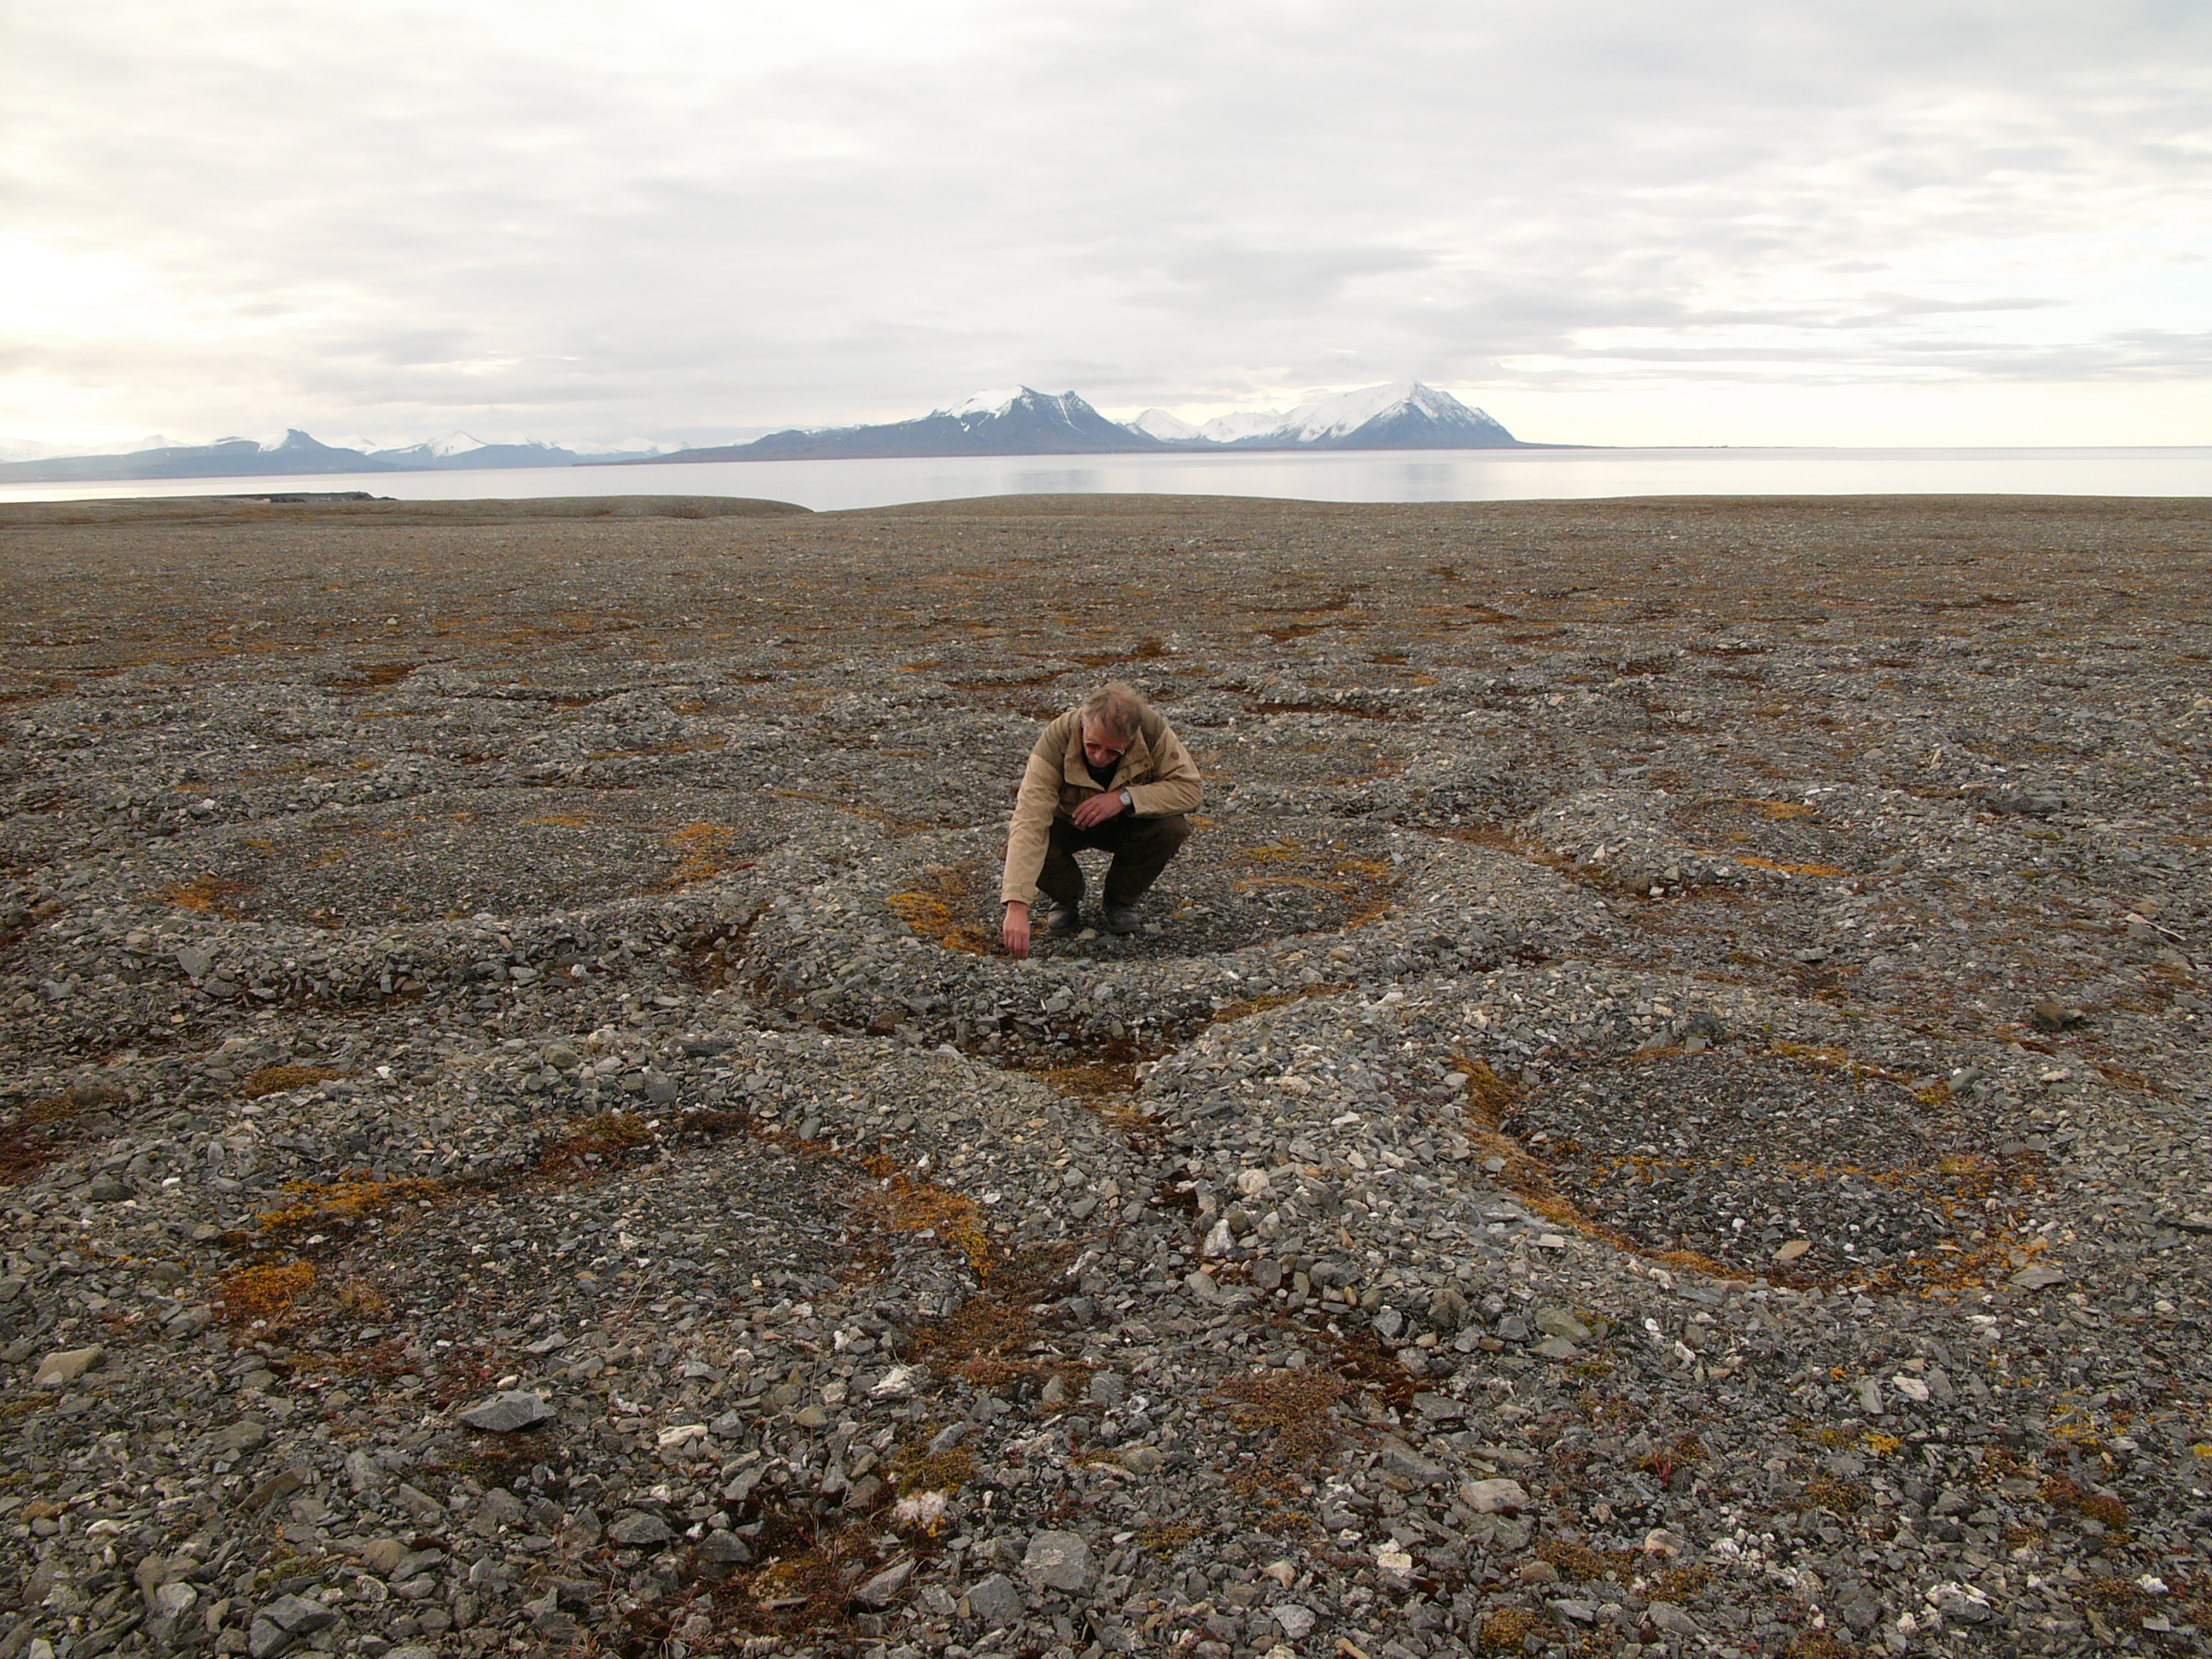
\includegraphics[trim=0 0 0.66\imagewidth{} 0, clip, width = 0.8\linewidth]{bilder/Permafrost_stone-rings_hg.jpg}
      \caption{Quelle: Wikimedia, Hannes Grobe}
    \end{figure}
    \column{.7\linewidth}
	\begin{itemize}
		\item Dauerhaft gefrorene Böden (permanent $<$ \SI{0}{\degreeCelsius})
		\item Größtenteils in Nordamerika und Eurasien
		\item Konserviert unzersetzte organische Materie
		\item [$\rightarrow$] Geschätzt 1000 Gt (1 Gt = $10^{15}$ g) Kohlenstoff gespeichert
		\item Deutliche Verschiebung der Permafrostgrenze im letzten Jahrhundert beobachtet
		\item Die globale Erwärmung gefährdet den Fortbestand des Permafrostes
		\item Folgen des Abtauens: Absenken der Böden, Überschwemmungen, Zersetzung bisher konservierter Materie
    \begin{itemize}
      \item[$\rightarrow$] Freisetzung großer Mengen CO$_2$ und Methan
    \end{itemize}
	\end{itemize}
\end{columns}

	\note{
		\begin{itemize}
			\item[] Tiefe des Permafrostes ist abhängig von Oberflächen-Temperatur
      \item[] Zum Teil mehrere hundert Meter tief gefroren
			\item[] In Sibirien liegt kaum Schnee, sodass die Böden noch kälteren Temperaturen ausgesetzt sind
			\item[] Verschiebung der Permafrost-Grenze in Kanada z.B um 100km nach Norden im letzten Jahrhundert
			\item[] Absinken gefährdet auch lokale Infrastruktur wie Straßen, Städte und Öl-Pipelines
			\item[] Überschwemmung gefährdet Wälder $\rightarrow$ 'ertrinken'
      \item[] Wissenschaft nimmt an, dass deutlich mehr Treibhausgase freigesetzt werden, als die erwartete neue Vegetation binden würde
		\end{itemize}
	}
\end{frame}

\begin{frame}
	\frametitle{Konsequenzen der Verringerung der Eismassen}
	\begin{itemize}
		\item Verringerter Albedo-Effekt
		\item Abgeschwächte Konvektion
		\item Abgeschwächte Ozeanströmung und Winde
		\item Anstieg des Meeresspiegels
		\item Massive Freisetzung von Treibhausgasen aus den Senken Ozean und Permafrost
		\item Trägheit führt zu verzögertem Eintreten der Änderungen
	\end{itemize}

	$\rightarrow$ Insgesamt: eine Verstärkung des Treibhauseffekt mit weiteren noch unabsehbaren Folgen

	\note{
		\begin{itemize}
			\item[] Das Schmelzen der Polkappen und Auftauen des Permafrostes ist ein deutliches Signal
			\item[] Wie gesagt, kann ein einmal in Gang gesetztes Abtauen schwer aufzuhalten sein
			\item[] Die Effekte können deutlich später auftreten
		\end{itemize}
	}
\end{frame}

\begin{frame}
	\frametitle{Vegetation}

	\begin{figure}
		\centering
		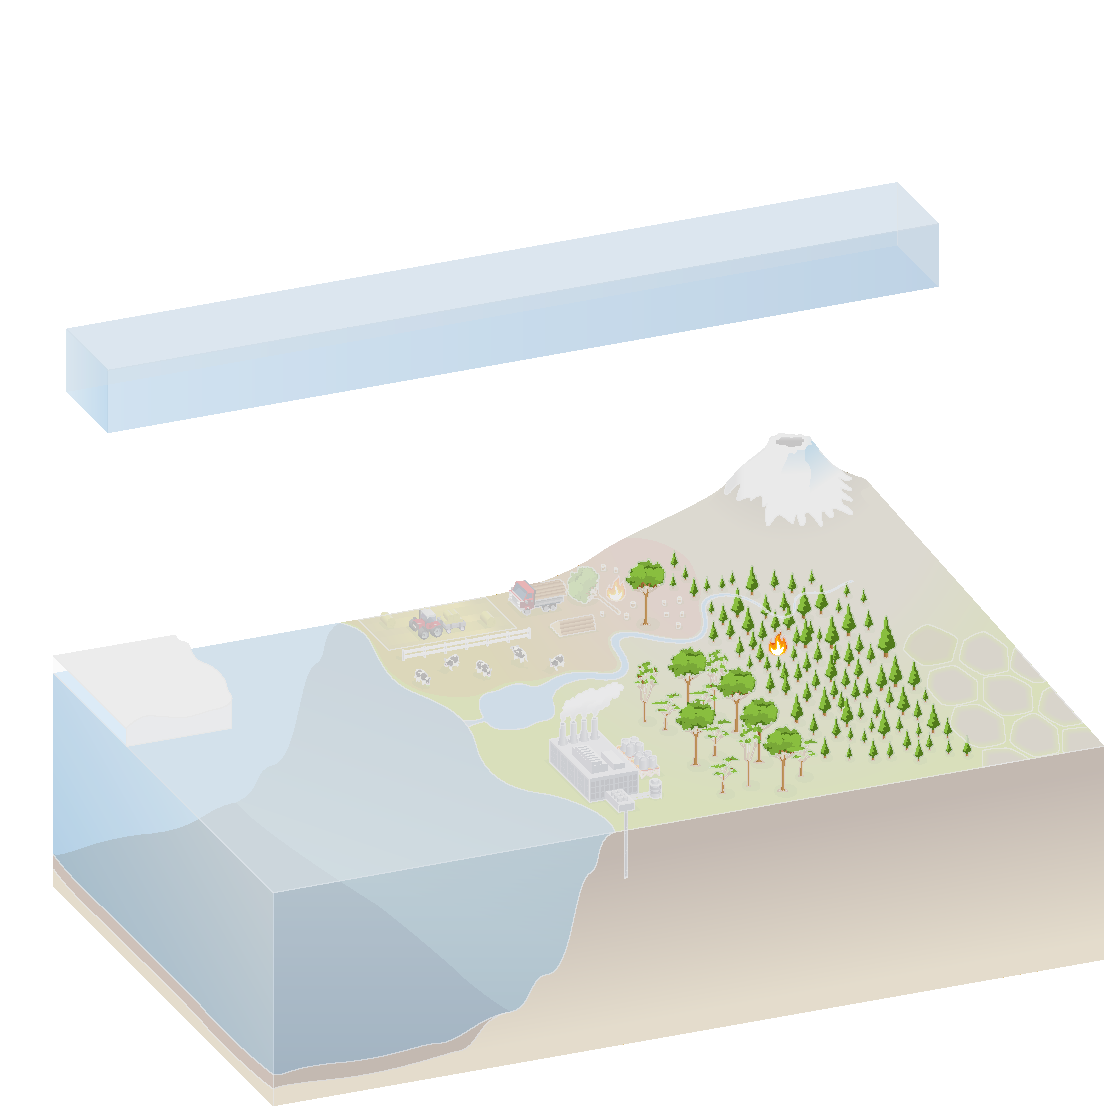
\includegraphics[trim={1cm 0cm 0cm 3cm}, clip, width=0.6\linewidth]{%
        bilder/climate_components/global_climate_components_biosphere.pdf}
		\caption{Die Vegetation ist eine interaktive Komponente des Klimasystems}
	\end{figure}

	\note{
		\begin{itemize}
			\item[] Vegetation ist sehr umfangreich und vielseitig
			\item[] steht in direktem Kontakt mit unterer Atmosphäre und Böden
			\item[] durch photosynthetische Prozesse und die Aufnahme sowie Abgabe von Wasser
			\item[] Vegetation hat dadurch massiven Einfluss auf Wetter und Klima - z.B. Tropischer Regenwald, Wolkenbildung
			\item[] zentral ist auch die Rolle beim Stoffkreislauf - u.a. Kohlenstoff, Phosphor, Nitrat, Stickstoff
			\item[] bietet Lebensraum und Lebensgrundlage
		\end{itemize}
	}
\end{frame}

\begin{frame}
	\frametitle{Pedosphäre - Böden}

	\begin{figure}
		\centering
		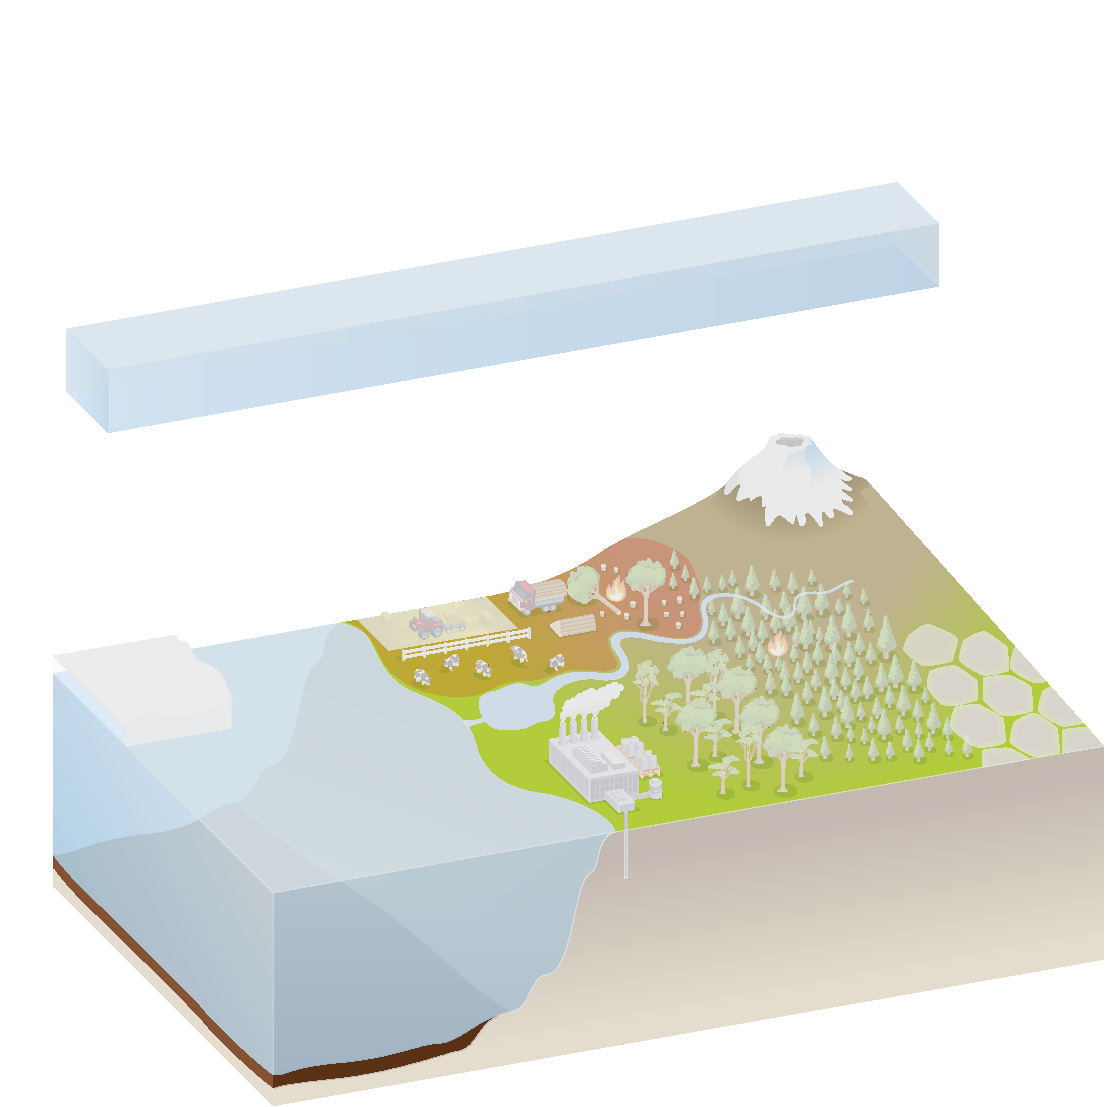
\includegraphics[trim={1cm 0cm 0cm 3cm}, clip, width=0.55\linewidth]{%
        bilder/climate_components/global_climate_components_pedosphere.pdf}
		\caption{Die Pedosphäre bezeichnet ist der Bereich der Erdoberfläche in dem sich Lithosphäre, Hydrosphäre, Atmosphäre und Biosphäre überschneiden.}
	\end{figure}

	\note{
		\begin{itemize}
			\item[] Boden
		\end{itemize}
	}
\end{frame}

\begin{frame}
	\frametitle{Lithosphäre - Gestein}

	\begin{figure}
		\centering
		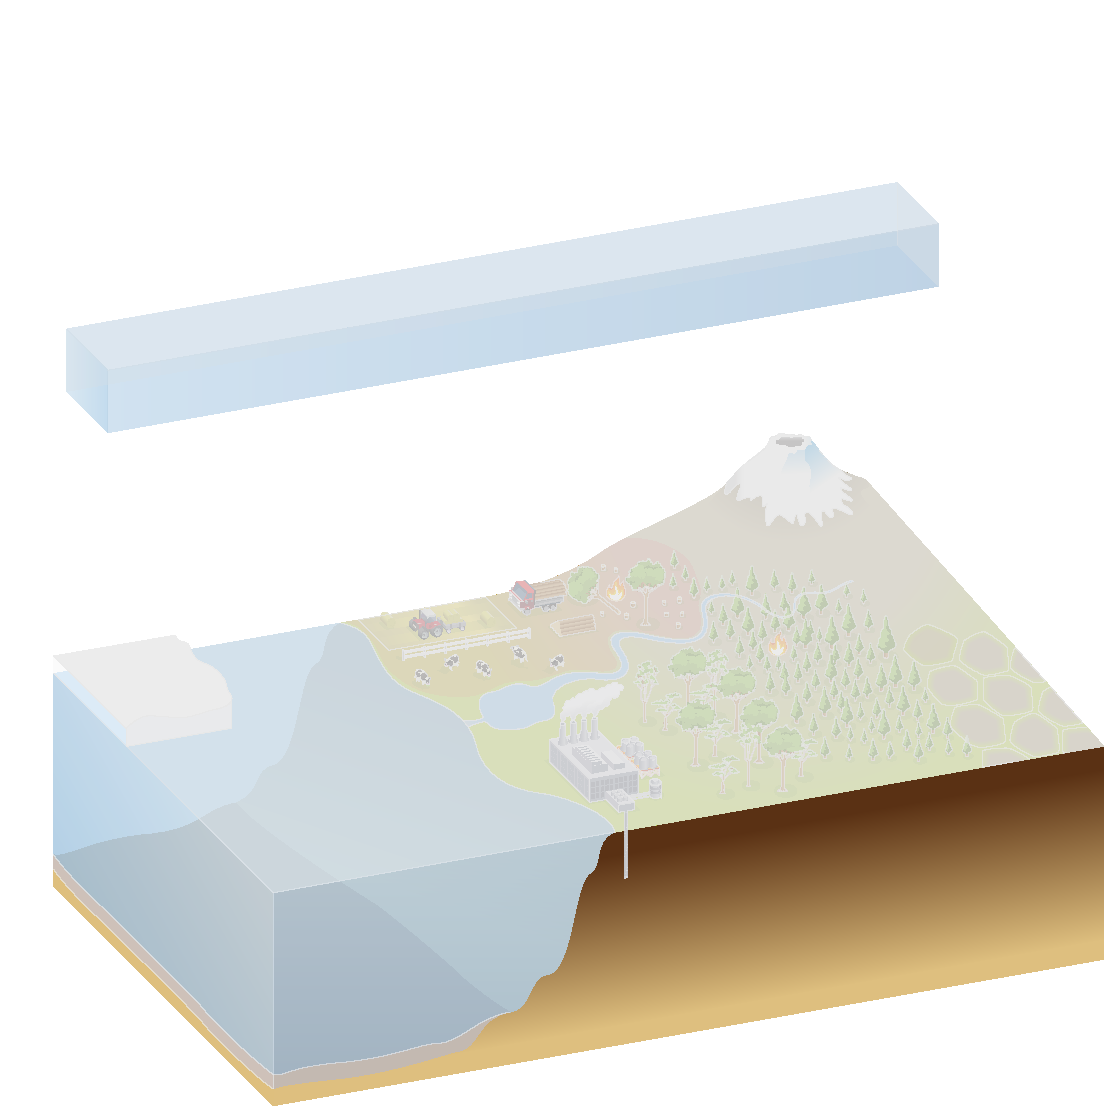
\includegraphics[trim={1cm 0cm 0cm 3cm}, clip, width=0.55\linewidth]{%
        bilder/climate_components/global_climate_components_lithosphere.pdf}
		\caption{Die Lithosphäre besteht aus der Erdkruste und dem relativ starren Teil des oberen Erdmantels.}
	\end{figure}

	\note{
		\begin{itemize}
			\item[] Gestein
		\end{itemize}
	}
\end{frame}

\subsection{Interaktionen der Faktoren des Klimasystems}
\begin{frame}
	\frametitle{Eis-Albedo-Rückkopplung}%Rahmstorf, Schellnhuber - Der Klimawandel S. 14
  \begin{center}
	 Reflexion der ankommenden Sonneneinstrahlung durch Eismassen\\[3em]
 \end{center}

	 \begin{columns}[T] % align columns
	 	\begin{column}{.48\textwidth}
	 		\centering
	 		\textbf{Abkühlung}\\
	 		\color{blue}\rule{\linewidth}{4pt}
	 		\color{black}
	 		\color<2->{gray}
	 		je mehr Eismassen\\
	 		$\downarrow$\\
	 		desto mehr wird reflektiert/\\
	 		desto weniger wird absorbiert\\
	 		$\downarrow$\\
	 		desto kälter wird es auf dem Planeten\\
	 		$\downarrow$\\
	 		desto weniger Wasserdampf kann die Atmosphäre aufnehmen\\
	 		$\downarrow$\\
	 		desto geringer wird der Treibhauseffekt
	 	\end{column}%
	 	\hfill%
	 	\begin{column}{.48\textwidth}<2->
	 		\centering
	 		\textbf{Aufwärmung}\\
	 		\color{red}\rule{\linewidth}{4pt}
	 		\color{black}
	 		je weniger Eismassen\\
	 		$\downarrow$\\
	 		desto weniger wird reflektiert/\\
	 		desto mehr wird absorbiert\\
	 		$\downarrow$\\
	 		desto wärmer wird es auf dem Planeten\\
	 		$\downarrow$\\
	 		desto mehr Wasserdampf kann die Atmosphäre aufnehmen\\
	 		$\downarrow$\\
	 		desto stärker wird der Treibhauseffekt
	 	\end{column}%
	 \end{columns}
\note{
\begin{itemize}
	\item[] hier wird die genannten Wechselwirkung unterschiedlicher Faktoren am Beispiel Eis-Albedo Rückkoppelung erläutert
	\item[] Albedo ist im wesentlichen das Reflexionsvermögen eines Körpers auf einer Skala von 0 bis 1, eine hohe Albedo bedeutet viel Reflexion
	\item[] I.a. gibt es viele ähnliche Rückkoppelungen im Klimasystem, z.B. auch bei Landnutzung/Grünflächen und kann im Prinzip sowohl positiv wie negativ sein
	\item[] Negative Rückkoplung führt zu einem stabilen Verhalten, positive Rückkopplung zu schwer kontrolierbarem Anwachsen.
  \end{itemize}
  }

\end{frame}

% "Runterscrollen" / "Zoom" in einer Abbildung von den Atmosphärischen Schichten auf die Erde

\begin{frame}
	\frametitle{Interaktion Hydrosphäre, Kryosphäre und Atmosphäre}
	\begin{columns}
		\column{.6\linewidth}
		\begin{figure}
			\centering
			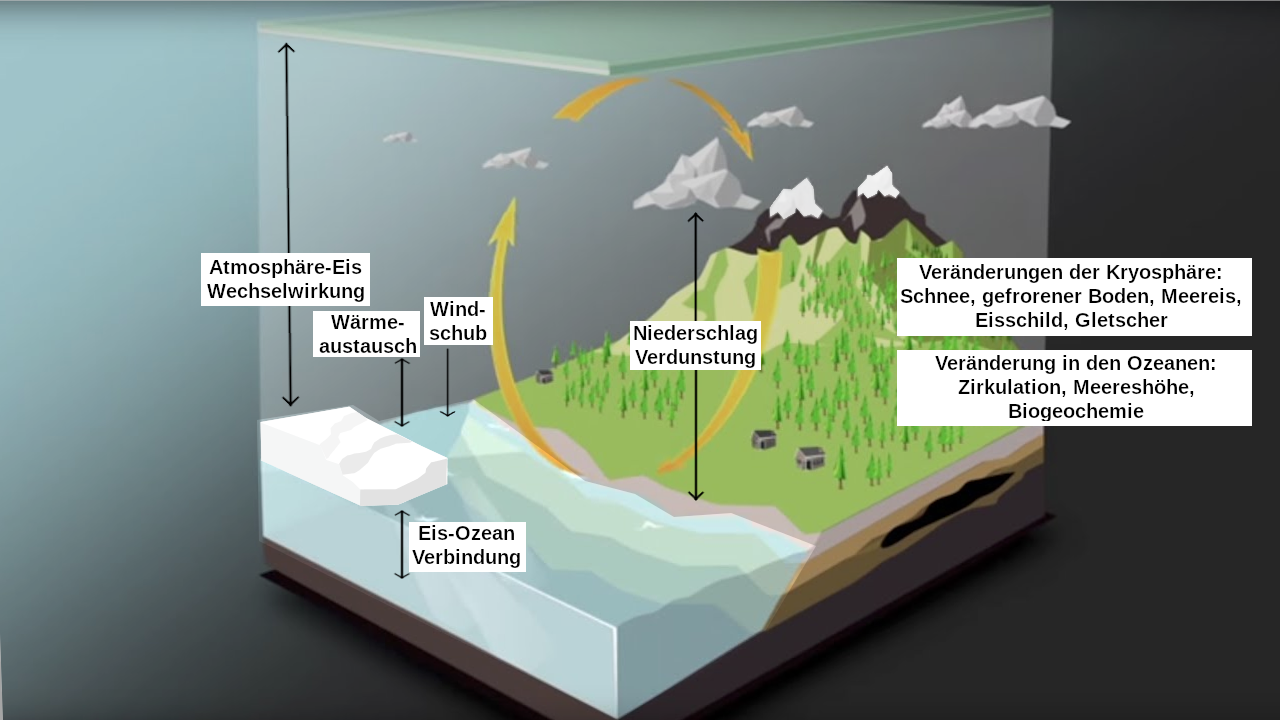
\includegraphics[width=\linewidth]{bilder/WMO_Cycles_factors_waterAndIce.png}
			\caption{Interaktion Hydrosphäre, Kryosphäre und Atmosphäre}
		\end{figure}
		\column{.4\linewidth}
		\begin{itemize}
			\item Verringerter Albedo-Effekt
			\item Abgeschwächte Konvektion
			\item Abgeschwächte Ozeanströmung und Winde
			\item Anstieg des Meeresspiegels
			\item Massive Freisetzung von Treibhausgasen aus den Senken Ozean und Permafrost
			\item Trägheit führt zu verzögertem Eintreten der Änderungen
		\end{itemize}
	\end{columns}
	\begin{block}{}
			$\rightarrow$ Insgesamt: eine Verstärkung des Treibhauseffekt mit weiteren noch unabsehbaren Folgen
	\end{block}

	\note{
		\begin{itemize}
			\item[] links an den Pfeilen sind die Wechselwirkungen notiert - z.B. Eis-Ozean-Verbindung (Konvektion)
			\item[] rechts sieht man die allgemeinen Elemente der Komponenten Hydrosphäre und Kryosphäre
			\item[] diese Elemente hängen offensichtlich zusammen und bedingen sich gegenseitig
			\item[] Das Schmelzen der Polkappen und Auftauen des Permafrostes ist ein deutliches Signal
			\item[] Wie gesagt, kann ein einmal in Gang gesetztes Abtauen schwer aufzuhalten sein
			\item[] Die Effekte können deutlich später auftreten
		\end{itemize}
	}
\end{frame}

\begin{frame}
	\frametitle{Interaktion Vegetation und Atmosphäre}

  \begin{figure}
    \centering
    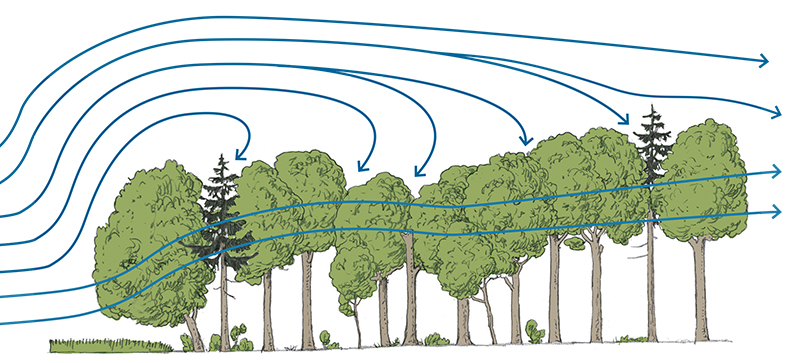
\includegraphics[width=.55\linewidth]{bilder/Wind_Vegetation.jpg}
    \caption{Wechselwirkung zwischen Atmosphäre und Biosphäre, Quelle: Stadt Kriens}
  \end{figure}
		\begin{itemize}
			\item Bodenbedeckung wirkt auf Wind, Wasseraustausch und Strahlungshaushalt
			\item [$\rightarrow$] Wälder bremsen Winde, speichern Wasser, beeinflussen Wolkenbildung und bilden Schatten und großen Lebensraum
			\item [$\rightarrow$] in Wüsten und Steppen versickert Wasser schneller und es gibt kaum Schatten, dafür existiert schwacher Albedo-Effekt
			\item Existenz und Wachstum von Vegetation bindet u.a. CO$_2$ und absorbiert Strahlung
			\item Absterben von Vegetation führt zu Freisetzung von CO$_2$ und anderen Stoffen in die Luft und Böden % Nitrat, Phosphat, Stickstoff etc.
		\end{itemize}

	\note{
		\begin{itemize}
			\item[] Photosynthese: Aufnahme von CO$_2$ und abgabe von O$_2$, Nutzung des Kohlenstoff für das Wachstum
			\item[] Lösung organischer Kohlenstoff-Verbindungen durch baterielle Zersetzung $\rightarrow$ Freisetzung von CO$_2$
			\item[] Änderungen an der Landoberfläche durch z.B: Änderung der Landnutzung - Waldrodung, Landwirtschaft ändern auch die Vegetation und die Ökosysteme
		\end{itemize}
		Fragen? Sonst $\rightarrow$ Klimamodelle
	}
\end{frame}

%\begin{frame}
%	\frametitle{Interaktion Vegetation und Atmosphäre}
%
%		\begin{figure}
%		\centering
%		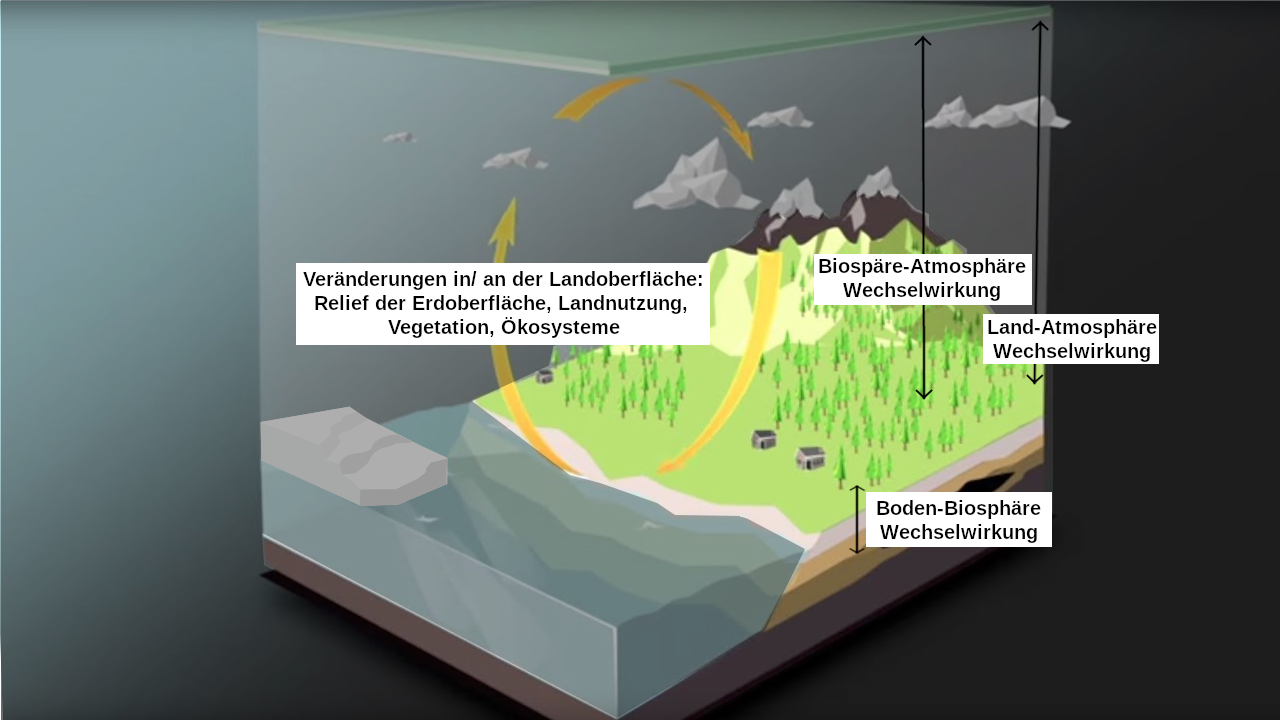
\includegraphics{bilder/WMO_Cycles_factors_landAndGround.png}
%		\caption{Interaktion der Biosphäre und Atmosphäre}
%	\end{figure}
%
%	\note{
%		\begin{itemize}
%			\item[] diesmal sind rechts die Wechselwirkungen der Vegetation und %Biosphäre zu sehen
%			\item[] links sind nochmal die zentralen Elemente der Komponente %Vegetation aufgelistet
%		\end{itemize}
%	}
%\end{frame}

